\documentclass[10pt,a4paper]{report}
\usepackage[english]{babel}
\usepackage{amsmath}
\usepackage{graphicx}
\usepackage{lmodern}
\usepackage[font=small,format=plain,labelfont=bf,up,textfont=it,up]{caption}
\usepackage[nottoc,notlof,notlot]{tocbibind}
\usepackage{url}
\usepackage{courier}
\usepackage[T1]{fontenc}
\usepackage[titles]{tocloft}
\usepackage{subcaption}
\usepackage{listings}
\usepackage{xcolor}
\usepackage[ruled,vlined]{algorithm2e}
\usepackage[toc,page]{appendix}
\usepackage{tocloft}

\setcounter{secnumdepth}{5}
\setlength{\parindent}{0in}

\renewcommand{\topfraction}{0.85}
\renewcommand{\textfraction}{0.1}
\renewcommand{\floatpagefraction}{0.75}

\definecolor{keyword}{RGB}{70,100,200}
\definecolor{kernel}{RGB}{139,0,0}
\definecolor{arrow}{RGB}{200,0,0}

\newcounter{ExamplesCounter}

\newcommand{\listexamplename}{List of Examples}
\newlistof{example}{ex}{\listexamplename}
\newcommand{\example}[1]{%
\refstepcounter{example}
%\par\noindent\textbf{Example \theexample. #1}
\addcontentsline{ex}{example}
{\protect\numberline{\thechapter.\theexample}#1}\par}

\newcommand{\listalgorithmslistname}{List of Algorithms}
\newlistof{algorithmslist}{alg}{\listalgorithmslistname}
\newcommand{\algorithmslist}[1]{%
\refstepcounter{algorithmslist}
%\par\noindent\textbf{Algorithm \thealgorithmslist. #1}
\addcontentsline{alg}{algorithmslist}
{\protect\numberline{\thechapter.\thealgorithmslist}#1}\par}

\def\nese{\mathrel{%
    \mathchoice{\NESE}{\NESE}{\scriptsize\NESE}{\tiny\NESE}%
}}
\def\NESE{{%
    \setbox0\hbox{$\nearrow$}%
    \rlap{\hbox to \wd0{\hss $\searrow$ \hss}}\box0
}}

\def\nesecol{\mathrel{%
    \mathchoice{\NESECOL}{\NESECOL}{\scriptsize\NESECOL}{\tiny\NESECOL}%
}}
\def\NESECOL{{%
    \setbox0\hbox{$\nearrow$}%
    \rlap{\hbox to \wd0{\hss \textcolor{arrow}{$\searrow$} \hss}}\box0
}}

\def\nwsw{\mathrel{%
    \mathchoice{\NWSW}{\NWSW}{\scriptsize\NWSW}{\tiny\NWSW}%
}}
\def\NWSW{{%
    \setbox0\hbox{\textcolor{arrow}{$\nwarrow$}}%
    \rlap{\hbox to \wd0{\hss $\swarrow$ \hss}}\box0
}}

\makeatletter
\newcommand\ackname{Acknowledgements}
\if@titlepage
  \newenvironment{acknowledgements}{
      \titlepage
      \null\vfil
      \@beginparpenalty\@lowpenalty
      \begin{center}%
        \bfseries \ackname
        \@endparpenalty\@M
      \end{center}}%
     {\par\vfil\null\endtitlepage}
\else
  \newenvironment{acknowledgements}{
      \if@twocolumn
        \section*{\abstractname}
      \else
        \small
        \begin{center}
          {\bfseries \ackname\vspace{-.5em}\vspace{\z@}}
        \end{center}
        \quotation
      \fi}
      {\if@twocolumn\else\endquotation\fi}
\fi
\makeatother

\title{Gene-Environment Interaction Analysis using GPU}
\author{Daniel Berglund}
\date{December 2014}

\begin{document}
\maketitle
\thispagestyle{empty}

\clearpage
\thispagestyle{empty}
\selectlanguage{english}
\begin{abstract}

\end{abstract}

\clearpage
\thispagestyle{empty}
\selectlanguage{english}
\begin{abstract}

\end{abstract}

%\clearpage
%\thispagestyle{empty}
%\begin{acknowledgements}
%Lorem ipsum
%\end{acknowledgements}

\clearpage
\tableofcontents
\thispagestyle{empty}

\clearpage
\setcounter{page}{1}
\chapter{Introduction}

\section{Outline}
The first chapter contains a short introduction to the area and the terminology. The second chapter gives the theoretical background. It starts with the statistics and algorithms and then describes the computer architecture and software design. The third algorithm section explains the structure of the current algorithms and also explains the design of the program that was developed in this thesis called CuEira. Section four provides the results and comparisons of the program performance. The fifth section is the discussion of these results. The last section discusses the future work.

%Aim of thesis

%TODO appendix contains bla bla

\section{Genome-wide association studies}
One type of study to find associations between genetic markers and diseases or other traits in different individuals is genome-wide association study(GWAS). Most GWAS do not study interactions between the genetic markers or between the genetic markers and environmental factors \cite{cordell_detect_review, gene_enviroment_2013}. Investigating gene-gene interactions recently has become more common\cite{cordell_detect_review}, however gene-environment interactions are still uncommon in studies\cite{gene_enviroment_2013}. Interactions between genes and environmental factors are considered to be important for complex diseases such as cancer or autoimmune diseases\cite{cordell_detect_review, gene_enviroment_2013, geira, ra_smoking}. In general a complex disease develops due to a combination of factors, not just a single gene or environmental factor\cite{rothman2008modern}. Examples of environmental factors are smoking, physical activity and so on.
\\
GWAS usually has a study design that is either cohort or case-control\cite{rothman2008modern}. In cohort study a sample of a population is followed and over time some individuals will develop the disease of interest\cite{mann_observational}. In case-control studies two groups are compared with each other to find the risk factors\cite{mann_observational}. One of these two groups consists of individuals with the disease and the other group consists of individuals similar to the first group but who do not have the disease\cite{mann_observational}.\\
\\
A typical GWAS consists of tens of thousands of individuals and up to several millions of genetic markers\cite{cordell_detect_review, burton2007genome}. In gene-gene interaction GWAS   few studies investigate more than the second order interaction because of the high number of possible combinations. There are some algorithms that can investigate higher order interactions however these have drawbacks\cite{gwis,high_order_2012,fast_high_order_cluster}.

%Problem vs gene-gene and gene-env
%focuses on gene-env, datatyp etc

\section{Genetics}
The genetic information is stored in \emph{chromosomes} each consisting of a \emph{DNA molecule}\cite{sadava_life}. Each chromosome comes in a pair where both chromosomes are nearly identical, except for the chromosomes related to gender\cite{sadava_life}. The DNA molecule is a double stranded helix of four nucleotide bases, \emph{adenine}(A),\emph{cytosine}(C),\emph{guanine}(G) and \emph{thymine}(T). They are always paired as A-T and G-C. \emph{Genes} are sections of these DNA molecules. The pair of genes in the chromosomes is a \emph{genotype}. The observable product of the genotype is called \emph{phenotype}, e.g. eye colour, fur patters.\\
\\
A position of the DNA or a gene is a \emph{locus}\cite{sadava_life}. A variation of the same gene or locus is an \emph{allele}\cite{sadava_life}. The effect of an allele on a phenotype can be either \emph{dominant}, \emph{recessive} or \emph{co-dominant}. Dominant means that if the allele is present the phenotype is expressed. For recessive the allele needs to be present in both chromosomes to be expressed\cite{sadava_life}. Co-dominant is when both alleles are expressed, when different alleles are present this usually produce some kind of intermediate state\cite{sadava_life}. An example of co-dominance is the human blood groups\cite{sadava_life}.

\begin{table}[h]
\begin{tabular}{| l l l |}
  \hline
  Genotype & Dominant & Recessive\\
  \hline
  AA & Effect & Effect \\
  GA & Effect & No Effect \\
  GG & No effect & No effect \\
  \hline  
\end{tabular}
\caption{The phenotype based on the genetic model and if the  allele with the effect is A}
\label{table:genetic}
\end{table}

\subsection{Major, Minor and Risk Allele}
\label{risk_allele}
The the allele that is least common using all individuals(both cases and controls) is the \emph{minor allele}, the one that is most common is the \emph{major allele}. The frequency of the minor allele is the \emph{minor allele frequency}(MAF)\cite{uvehag_master_thesis, geira}. If the MAF is too low an analysis often will be of little value so all SNPs with MAF below a threshold are usually skipped. 5\% is common value of the threshold\cite{burton2007genome, geira}.\\
\\
To determine if the genetic risk is present for each individual one of the alleles needs to be chosen as the \emph{risk allele}. GEIRA and JEIRA defines the risk allele as the minor allele in cases if the MAF of cases is greater than the MAF of controls, otherwise the major allele in cases is used\cite{geisa, uvehag_master_thesis}. However JEIRA and GEISA does not calculate the risk allele according to that definition, see appendix \ref{risk_allele_appendix} for the details. In this thesis the risk allele will be defined as the allele that has higher frequency in cases than controls. It is similar to the definition using MAF in most cases. Appendix \ref{risk_allele_appendix} has more detailed comparisons.\\
\\
The presence of genetic risk based on the risk allele and the genetic model can be coded as a variable than then be can used in a statistical model. For dominant or recessive genetic model this means that the variable is binary since the risk is either present or not\cite{geira}. See table \ref{table:genetic} for how the coding is based on the model. For co-dominant model the number of risk alleles in the individual is used as the variable, 0, 1 or 2 \cite{geira}.

\section{Defining Interaction}
\label{interaction}
There are several ways to define interaction. The overall goal is often to detect if \emph{biological} interactions are present. \emph{Biological} interaction is when different factors co-operate through a physiological or biological mechanism and cause the effect, e.g. the disease. The information about the factors can then be used to explain the mechanisms involved in causing the disease and possibly help to find cures for them. However biological interaction is not well defined and thus it is not possible to calculate it directly from data.\cite{interaction_confusion, rothman2008modern,rothman2002intro_epidemiology}\\
\\
That is why statistical interaction is used and it is assumed that the presence of statistical interaction implies the presence of biological interaction

\emph{Statistical} interaction on the other hand is well defined. However it is scale dependent, i.e. interactions can appear and disappear based on transformations of the given data. Statistical interaction also depends on the model used. The common way to define statistical interaction is to consider the presence of a product term between the variables in the model, this is referred to as \emph{multiplicative} interaction. For instance for a linear model
\begin{equation}
f(x,y)=ax+by+cxy+d
\end{equation}
$c$ is the product term that represents multiplicative interaction between variables x and y so the test for multiplicative interaction is to test if c=0 \cite{geira, interaction_confusion, rothman2008modern}. In some cases it is instead tested as a=b=c=0, this is testing for \emph{association allowing for interaction}\cite{cordell_detect_review}.\\
\\
\emph{Additive} interaction is another kind of statistical interaction that is broader than multiplicative interaction. It is when the total effect of the interacting factors present is larger than the sum of their separate effects. A more precise definition can be found in section \ref{additive}. It implies biological interaction as defined by Rothman\cite{rothman2008modern}, which is sometimes called \emph{causal interdependence} or \emph{causal interaction}\cite{causal_bounds_arvid}. Additive interaction can find more possible interactions than multiplicative and since it is closer to biological interaction it is often chosen in epidemiological studies\cite{interaction_confusion}.  

\section{GEIRA, JEIRA and GEISA, the Aim of the Project}
\label{jeira}
To search for interaction in data various tools can be used. \emph{GEIRA}\cite{geira} is one such tool which uses logistic regression, additive interaction and with bootstrap to asses the quality of the models\cite{geira}. It comes in two versions, one made in R and one in SAS. To improve speedup it was later implemented in Java and called \emph{JEIRA}\cite{uvehag_master_thesis}. It is parallel which made it significantly faster\cite{uvehag_master_thesis}. \emph{GEISA}\cite{geisa} is another tool based on JEIRA however it uses permutation testing instead of bootstrap to asses the certainty of the models\cite{geisa}. The programs structure is explained in section \ref{implementation}, the algorithms are explained in section \ref{algorithm_background}. Bootstrap calculates the certainty by resampling the data\cite{agresti_categorical}. Permutation tests works in a similar way but only randomizes the outcomes \cite{lindgren1993statistical}.\\
\\
The aim of this project is to make the gene-environment interaction analysis faster by using graphics processors and to be able to handle larger amounts of data. The program is written in C++ and CUDA.

%\\
%The genetic markers mentioned previously are commonly single nucleotide polymorphism(SNP, pronounced snip). SNPs are variations in the genome where a single nucleotide is different %between individuals in a population\cite{sadava_life}.\\

\clearpage
\chapter{Background}
This section will go through some of the background starting with the statistical background, continuing with computer architecture and software design after that. Last is a section about the algorithms.

\section{Statistical Background}
This section will explain some of the statistical background of categorical statistics.

\subsection{Contingency Tables}
A contingency table is a matrix used to describe categorical data. Each cell contains a count of occurrences for a specific combination of variables. Table \ref{table:contingency_table} is an example of an 2 x 2 table. From this table we can for instance see that 688 smokers got lung cancer. Contingency tables are the basis for various statistical tests to model the data.\cite{agresti_categorical}

\begin{table}[h]
\begin{tabular}{| l c c |}
  \hline
  & Lung cancer & No lung cancer\\
  \hline
  Smoker & 688 & 650 \\
  Non smoker & 21 & 59 \\
  \hline  
\end{tabular}
\caption{Contingency table describing the outcome of a study, from \cite{agresti_categorical}, page 42}
\label{table:contingency_table}
\end{table}

\subsection{Relative Risk and Odds Ratio}
\label{rr_or}
From a contingency table it is possible to calculate some useful measures such as the risk of getting the outcome based on exposure. The risk for a row $i$ in the table will be referred to as $\pi_i$. For table \ref{table:contingency_table} the risks $\pi_1$ and $\pi_2$ is

\begin{equation}
\pi_1=\frac{688}{688+650}=0.51
\end{equation}

\begin{equation}
\pi_2=\frac{21}{21+59}=0.36
\end{equation}

To compare different risks, for instance between smokers and non smokers, the ratio of the risks is used\cite{agresti_categorical}. It is called \emph{relative} risk(RR) is defined as\cite{agresti_categorical} 

\begin{equation}
RR=\frac{\pi_1}{\pi_2}
\end{equation}

So for the table \ref{table:contingency_table} the relative risk of getting lung cancer based on exposure to smoking is

\begin{equation}
RR=\frac{0.52}{0.36}=1.96
\end{equation}

This means that the risk of getting lung cancer for a smoker is almost twice as high for a non smoker in this data.

Another useful measure is \emph{odds} and \emph{odds ratio}(OR). The odds is\cite{agresti_categorical} 

\begin{equation}\label{eq:odds}
\Omega=\frac{\pi}{1-\pi}
\end{equation}

The odds are non-negative and $\Omega>1$ when the outcome is more likely than not\cite{agresti_categorical}. So for $\pi=0.75$ the odds is $\Omega=\frac{0.75}{1-0.75}=3$. This means that the outcome is 3 times more likely to occur than not. ORs can be used as an approximation of RR in case control studies because RR can not be estimated in that type of studies\cite{or_mislead}. Cohort studies on the other hand can give estimates of RR\cite{or_mislead}. OR is the ratio of the odds just as RR is the ratio of the risks\cite{agresti_categorical}.

\begin{equation}\label{eq:odds_ratio}
\theta=\frac{\Omega_1}{\Omega_2}
\end{equation}

In the case when the outcome is a disease or similar variables with odds ratio below one are called \emph{protective} and when it is above one it is a \emph{risk factor}\cite{recoding_2011}.

\subsection{Additive Interaction}
\label{additive}
Interaction was talked about in section \ref{interaction}. The more precise definition of additive interaction is the divergence from additive effects on a logarithmic scale, e.g\cite{rothman2008modern}.

\begin{equation}
OR_{both\:factors\:present}>OR_{first\:factor\:present}+OR_{second\:factor\:present}-1
\end{equation}

A third variable is used to model the interaction for both multiplicative and additive interaction. Multiplicative interaction as explained in section \ref{interaction} does not include the effects from the factors, i.e. the main effects, in the interaction variable. However for additive interaction the interaction variable models the whole effect including the main effects. This means that the third variable for multiplicative and additive interaction are identical, however for additive interaction the first and second variable is zero when both factors are present. The coding for additive interaction is summarized in table \ref{table:coding}\cite{uvehag_master_thesis}.

\begin{table}[h]
\begin{tabular}{| l | c c c|}
  \hline
  Factor present & First variable & Second variable & Interaction \\
  \hline
  None & 0 & 0 & 0 \\
  \hline 
  First & 1 & 0 & 0 \\
  \hline
  Second & 0 & 1 & 0 \\
  \hline
  Both & 0 & 0 & 1 \\
  \hline
\end{tabular}
\caption{Coding of the variables for LR}
\label{table:coding}
\end{table}

\subsection{Statistic Measures for Additive Interaction}
\label{statistic_measures}
Based on the statistical model and its corresponding ORs there are some measures that can be calculated. These measures show various properties of the additive interaction. They are defined using $RR$ however as mentioned before in section \ref{rr_or} $OR$ can be used to approximate $RR$.\\
\\
\emph{Relative  excess risk due to interaction}(RERI) is how much of the risk is due to interaction\cite{rothman2008modern, recoding_2011}. It is defined as\cite{rothman2008modern, recoding_2011}
\begin{equation}
RERI=RR_{11}-RR_{10}-RR_{01}+1
\end{equation}

\emph{Attributable proportion due to interaction}(AP) is similar to RERI however is the proportion relative to the interaction relative risk\cite{rothman2008modern, recoding_2011}.
\begin{equation}
AP=\frac{RERI}{RR_{11}}=\frac{1}{RR_{11}}-\frac{RR_{10}}{RR_{11}}-\frac{RR_{01}}{RR_{11}}+1
\end{equation}

\emph{Synergy index}(SI) is the ratio of the combined effects and the individual effects\cite{rothman2008modern, recoding_2011}.
\begin{equation}
\frac{RR_{11}-1}{RR_{10}+RR_{01}-2}
\end{equation}

By using the definition of additive interaction it can be shown that additive interaction is present when $RERI>0$, $AP>0$ and $SI>0$\cite{recoding_2011}.

\subsubsection{Recoding of Protective Effects}
\label{recode}
The measures for additive interaction RERI, AP and SI explained in the previous section are developed for risk factors, i.e. $OR>1$, which causes problems if a factor is protective\cite{recoding_2011}. This can be solved by \emph{recoding}, it switches the group of individuals without both factors, i.e. the \emph{reference group}, with the group that has the lowest  $OR$\cite{recoding_2011}. There are three possible combinations of the factors excluding the reference group shown in table \ref{table:recoding_cases}. Switching a group changes the level of the factors for all in individuals in the group to the reference groups level, and switches the individuals in the reference group with the groups level.

\begin{table}[h]
\begin{tabular}{| l l l |}
  \hline
  Genetic factor & Environment factor & Recoding case\\
  \hline
  0 & 0 & N/A \\
  1 & 0 & 1 \\
  0 & 1 & 2 \\
  1 & 1 & 3 \\
  \hline
\end{tabular}
\caption{Cases of recoding}
\label{table:recoding_cases}
\end{table}

\subsection{Confounders and Covariates}
\emph{Confounding} is one of the central issues in design of epidemiological studies. It is when the effect of the exposure is mixed with the effect of another variable. So if we do not measure the second variable, the effect of the first would be estimated as stronger than it really is. The second variable is then a \emph{confounder}. Several methods in epidemiology are about avoiding or adjusting for confounding. Sometimes these variables needs to be incorporated into the models. \emph{Covariates} are possible confounders or other variables that one wants to adjust for in the model. Sometimes covariates are called \emph{control variables}.\cite{rothman2002intro_epidemiology,rothman2008modern}

\begin{figure}[h]
    \centering
    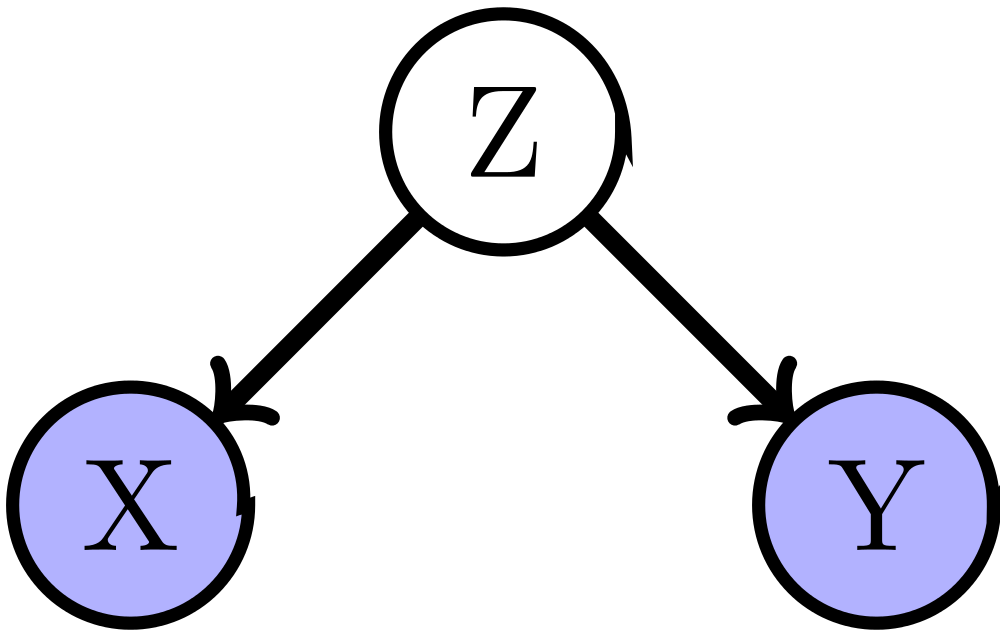
\includegraphics[width=5cm]{Simple_Confounding_Case.png}
    \caption{Illustration of a simple case of confounding. If we do not observe Z we might falsely find an association between X and Y}
    \label{fig:confunding}
\end{figure}

For instance if a study would look into the effects of yellow teeth on lung cancer they would likely find an effect. However it would be due to the confounder smoking since smoking causes yellow teeth and lung cancer\cite{smoking_teeth}.

\subsection{The Multiple Testing Problem}
It is not uncommon to test many hypothesis on the same data and in the case of GWAS it can be billions of tests. If one continues to test one should eventually find something that is significant due to random chance. With the common significance threshold of 5\% it is expected to get 1 in 20 false positives under the assumption that the null hypothesis is true. The problem arises from the fact that the hypothesis tests are dependent on each other since they use parts of the same data. This is the multiple testing problem and if it is not corrected for many false positives might be found.\cite{bonferroni_multiple}\\
\\
Bonferroni correction is the simplest method and viewed as a conservative way to correct for this problem. It simply divides the significance threshold by the number of hypothesis tested. However the number of hypothesis made is not always clear. With a two-stage analysis, is the number of hypothesis the number of tests done in both stages combined, the number made in the first stage or the second stage?\cite{bonferroni_multiple}

\section{Computer Architecture Background}
This section explains some of the computer architectures used to perform tasks in a thesis. A large part of this chapter is focused on the optimization techniques that are in use. For the purpose of this thesis it is best to think of the computer consisting of four main parts, the processor, the data storage, the memory and the accelerator.

\subsection{Central Processing Unit}
Central processing unit(CPU) is the part of the computer that executes instructions one by one\cite{introduction_hpc_hager}. Most modern CPUs have multi-core architecture meaning they consist of several processors\cite{introduction_hpc_hager}. Each core can perform tasks independent of each other. Multi-core architecture affects the way the programs are made because they need to be parallel to get maximum speed. More about this in section \ref{concurrency}.
\\
The figures \ref{fig:cpu_scheme} and \ref{fig:core_die} shows how the CPU is divided into areas and that most of it is not used for calculations. A large part of the area is used for various optimizations.

\begin{figure}[h]
    \centering
    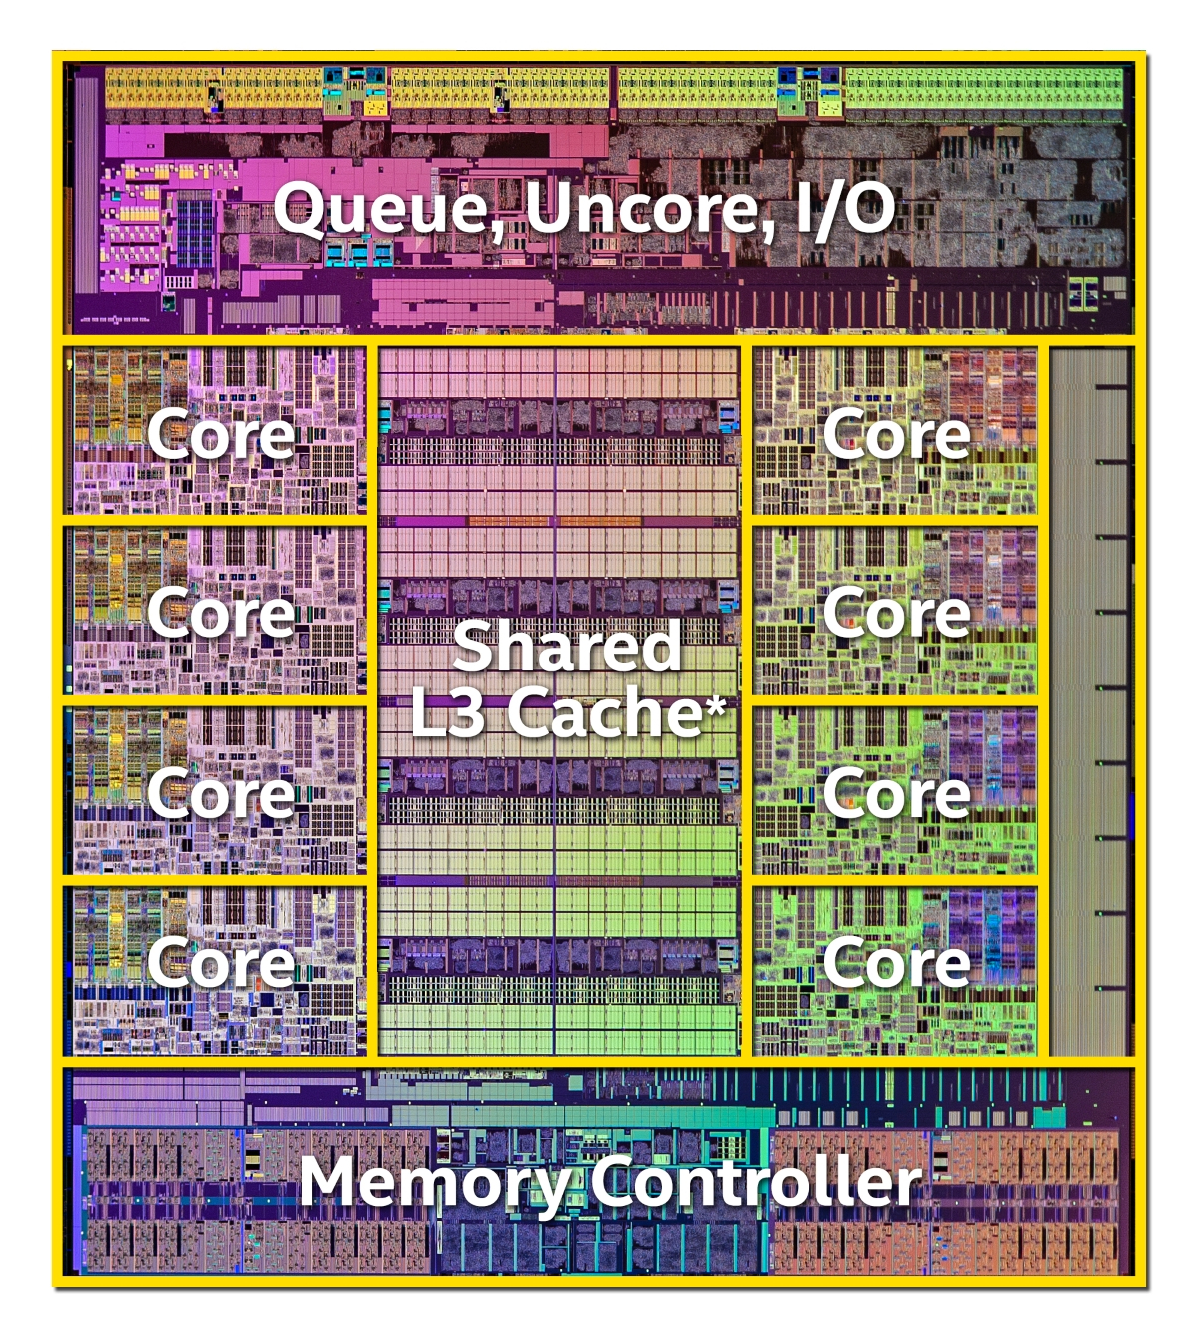
\includegraphics[width=7cm]{cpu_scheme_haswell.jpg}
    \caption{The layout of the Haswell architecture i7-5960x, from \cite{intel_haswell_2014}}
    \label{fig:cpu_scheme}
\end{figure}

\subsection{Concurrency and Threads}
\label{concurrency}
\emph{Concurrency} means doing multiple things and the same time, instead of \emph{sequential}. This can cause various problems such as the same object being accessed at the same time. The dinning philosophers is an concurrency problem that can used to illustrate some of these problems. A group of philosophers is sitting at a round table, each has a plate of spaghetti in front of them and there is a fork between each pair of philosophers\cite{hoare1985communicating}. The philosophers alternate between thinking and eating. However they can only eat if they have both the right and left fork\cite{hoare1985communicating}.

\begin{figure}[h]
    \centering
    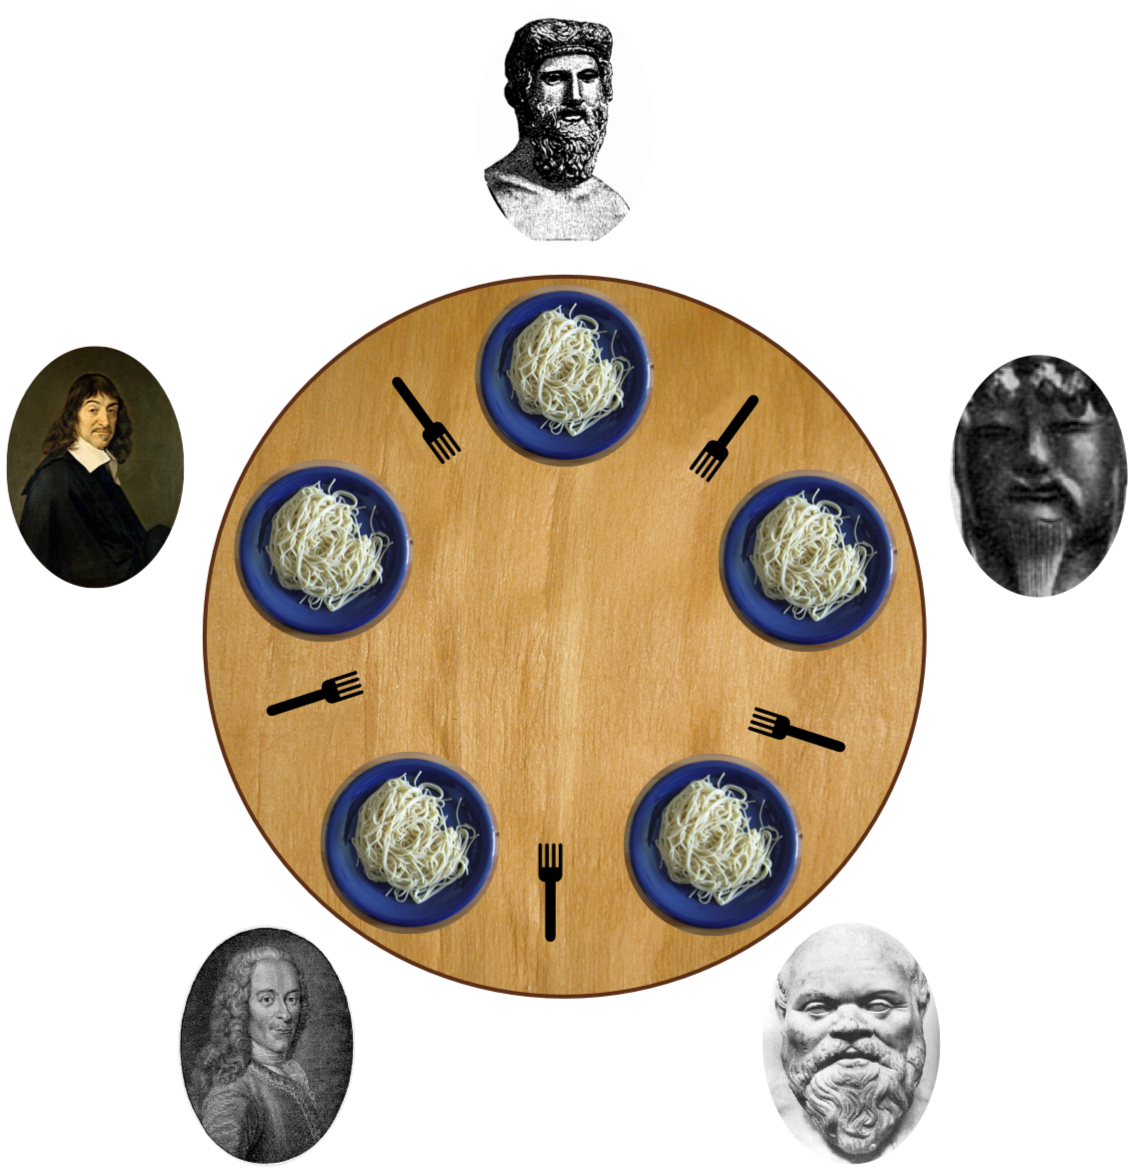
\includegraphics[width=5cm]{dining_philosophers.png}
    \caption{Illustration of the dining philosophers problem. Wikipedia Commons}
    \label{fig:dining_philosophers}
\end{figure}

A potential proposal\cite{hoare1985communicating} for behaviour instructions could be:
\begin{itemize}
 \item Think
 \item Wait for a fork to become available and pick up that fork
 \item Wait for and pick up the other fork
 \item Eat
 \item Put down the forks one by one
 \item Go back to thinking
\end{itemize}
The problem is that this set of instructions can lead to a state where everyone is holding one fork and waiting to get the other one\cite{hoare1985communicating}. But no one is done eating so no forks will become available. The system is then locked into its state, this is called a \emph{deadlock}\cite{hoare1985communicating, introduction_hpc_hager}. A potential solution to the problem in this case is to introduce a person that dictates if a philosopher is allowed to eat or not\cite{hoare1985communicating}.\\
\\
There are also other potential problems that can arise when using concurrency. A \emph{race condition} occurs when the result depends on what affects it first, it is a race between them on who can reach it first\cite{introduction_hpc_hager}. \emph{Locks} can be used to prevent situations as the ones described above by making sure only one thread at a time can access the object\cite{introduction_hpc_hager}.

In computer science concurrency occurs when instructions are separated in different \emph{threads}. The architectures can be divided in a taxonomy with four categories including the sequential. They are illustrated in figure \ref{fig:flynn_taxonomy}.

\begin{itemize}
 \item \emph{SISD}(Single-Instruction,Single-Data) is the sequential and is as the name says, single instructions on single data\cite{introduction_hpc_hager}.
 \item \emph{SIMD}(Single-Instruction, Multiple-Data) is applying the same instruction on different data\cite{introduction_hpc_hager}. SIMD is also called vectorisation\cite{introduction_hpc_hager}.
 \item \emph{MIMD}(Multiple-Instruction, Multiple-Data) applies different instructions on different data\cite{introduction_hpc_hager}.
 \item \emph{MISD}(Multiple-Instruction, Single-Data) performs different operations at the same piece of data, this paradigm is uncommon\cite{introduction_hpc_hager, computer_arch_2003}.
\end{itemize}

\begin{figure}
        \centering
        \begin{subfigure}[b]{0.48\textwidth}
                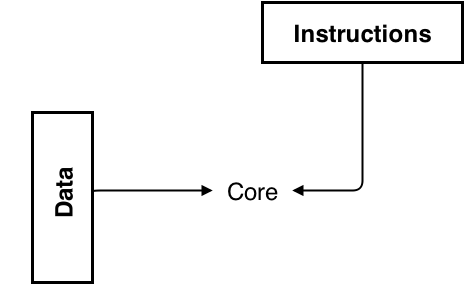
\includegraphics[width=\textwidth]{SISD}
                \caption{SISD}
                \label{fig:SISD}
        \end{subfigure}%
        ~
        \begin{subfigure}[b]{0.48\textwidth}
                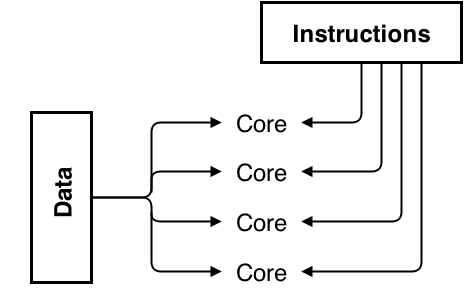
\includegraphics[width=\textwidth]{MISD}
                \caption{MISD}
                \label{fig:MISD}
        \end{subfigure}

        \begin{subfigure}[b]{0.48\textwidth}
                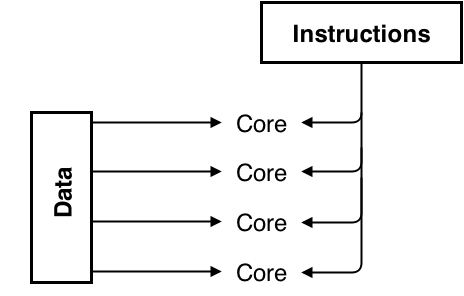
\includegraphics[width=\textwidth]{SIMD}
                \caption{SIMD}
                \label{fig:SIMD}
        \end{subfigure}
        ~
        \begin{subfigure}[b]{0.48\textwidth}
                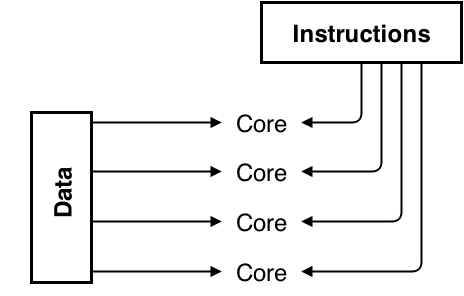
\includegraphics[width=\textwidth]{MIMD}
                \caption{MIMD}
                \label{fig:MIMD}
        \end{subfigure}
        \caption{Flynns taxonomy of parallel architectures\cite{introduction_hpc_hager}}\label{fig:flynn_taxonomy}
\end{figure}

\subsection{Memory, Caching and Optimizations}
\label{optimizations}
Various optimizations have been introduce to the CPUs over the years\cite{drepper2007cpumemory, introduction_hpc_hager}. Some are common and almost all CPUs have them, others are unique to a specific vendor or CPU\cite{introduction_hpc_hager}. Figure \ref{fig:core_die} show the layout of a CPU core. This section explains some of the more common optimizations.

\begin{figure}[h]
    \centering
    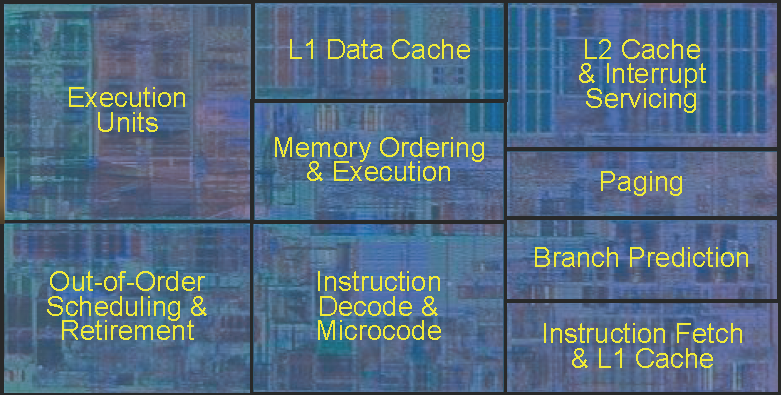
\includegraphics[width=8cm]{cpu_core_die.png}
    \caption{Layout of a CPU core, Intel Nehalem i7, from \cite{tomshardware_nehalem}}
    \label{fig:core_die}
\end{figure}

In general retrieving data from memory is relatively slow compared to how fast the processor works\cite{introduction_hpc_hager,drepper2007cpumemory}. To solve this problem a \emph{cache} was introduced\cite{drepper2007cpumemory}. It stores recently used data in a very small and very fast memory that resides on the CPU chip itself\cite{drepper2007cpumemory}. The caches varies in sizes, the latest ones are around 16-20 mB, for instance Intels i7-5960x with 20 mB \cite{intel_haswell_2014_5960x}. The cached data can then be reused without waiting for the main memory to fetch it. However when the data is not in the cache it costs time to fetch it from the main memory, that is a \emph{cache miss}\cite{drepper2007cpumemory}. Avoiding cache misses is important for the speedup\cite{drepper2007cpumemory}. Modern CPUs commonly have more than one cache, most have three\cite{introduction_hpc_hager}. They are named L1 to L3, with L1 being the one fastest and smallest and L3 the largest and slowest\cite{introduction_hpc_hager}.\\
\\
Modern multi-core processors have several L1 caches, one per core\cite{introduction_hpc_hager}. Commonly each core has a L2 cache as well, however it can be shared in some architectures\cite{introduction_hpc_hager}. The L3 cache is almost always shared between all cores\cite{introduction_hpc_hager}. The multiple caches used causes a problem called \emph{cache coherency}. It is when the data modified in one cache needs to be updated in all the caches in order for them to use the new value\cite{introduction_hpc_hager}.\\
\\
One of the memory optimization methods somewhat related to caches is \emph{prefetching}\cite{introduction_hpc_hager, drepper2007cpumemory}. Instead of fetching just the data requested by the current operations it also fetches the surrounding data\cite{drepper2007cpumemory}. Even if the data is not needed at the given point in time, the chance that the surrounding data will be used soon is high since it is common to iterate over arrays and similar structures\cite{introduction_hpc_hager}.\\
\\
When a program iterates over an array the first value is a cache miss since it is not in the cache. The following values are prefected and cached as well. However if the array is too long to be prefetched and cached completely and the CPU hits a position not in the cache then a new cache miss happens\cite{drepper2007cpumemory}. Usually matrices are stored sequential in memory\cite{drepper2007cpumemory}. For instance a two dimensional matrix is stored as a one dimensional array. Different programming languages store them differently, either column by column or row by row\cite{drepper2007cpumemory}. Row by row is called \emph{row major} and column by column is \emph{column major.}\\
\\
Below is an example of how prefectching can have an large impact on performance.\\
\\
In section 6.2.1 in What Every Programmer Should Know About Memory\cite{drepper2007cpumemory} an example of how much speed that can be gained by optimizing matrix matrix multiplication. The variables have been renamed for clarity. The simple version of it is shown in algorithm \ref{alg:matmatmult} and the version with improved cache use is shown in \ref{alg:matmatmultopt}.

\begin{algorithm}
\DontPrintSemicolon
\SetStartEndCondition{ (}{)}{)}\SetAlgoBlockMarkers{\{}{\}}%
\SetKwProg{Fn}{}{}{}\SetKwFunction{FRecurs}{void FnRecursive}%
\SetKwFor{For}{for}{}{}%
\SetKwIF{If}{ElseIf}{Else}{if}{}{elif}{else}{}%
\SetKwFor{While}{while}{}{}%
\SetKwRepeat{Repeat}{repeat}{until}%
\AlgoDisplayBlockMarkers\SetAlgoNoLine%

\SetKwInOut{data}{Data}
\BlankLine \BlankLine

\data{Three $N \times N$ matrices, \textit{matrix1}, \textit{matrix2} and \textit{result}}

\BlankLine \BlankLine
\For{i = 0; i < N; ++i}{
  \For{j = 0; j< N; ++j}{
    \For{k = 0;k < N; ++k}{
      $result[i][j]+= matrix1[i][k] * matrix2[k][j]$;\;
    }
  }
}

\caption{Basic algorithm for matrix matrix multiplication of two $N \times N$ matrices}
\algorithmslist{Basic algorithm for matrix matrix multiplication of two $N \times N$ matrices}
\label{alg:matmatmult}
\end{algorithm}

By transposing the mul2 matrix it becomes more cache friendly by using prefectching of surrounding data the way that mul1 already is\cite{drepper2007cpumemory}. The transpose itself can be eliminated while also making it use the cache better by reading in the correct amount of data, this is the size SM in the code\cite{drepper2007cpumemory}. The optimized version is shown in \ref{alg:matmatmultopt}. It took 17.3\% of the original time\cite{drepper2007cpumemory}.

\begin{algorithm}
\DontPrintSemicolon
\SetStartEndCondition{ (}{)}{)}\SetAlgoBlockMarkers{\{}{\}}%
\SetKwProg{Fn}{}{}{}\SetKwFunction{FRecurs}{void FnRecursive}%
\SetKwFor{For}{for}{}{}%
\SetKwIF{If}{ElseIf}{Else}{if}{}{elif}{else}{}%
\SetKwFor{While}{while}{}{}%
\SetKwRepeat{Repeat}{repeat}{until}%
\AlgoDisplayBlockMarkers\SetAlgoNoLine%

\SetKwInOut{data}{Data}
\BlankLine \BlankLine

\data{Three $N \times N$ matrices, \textit{matrix1}, \textit{matrix2} and \textit{result}\\
$SM$ is the number of matrix elements that fits in the cache.
}

\BlankLine \BlankLine

\For{i = 0; i < N; i += SM}{
  \For{j = 0; j < N; j += SM}{
    \For{k = 0; k < N; k += SM}{
      \For{i2 = 0, rresult = \&result[i][j], rmatrix1 = \&matrix1[i][k]; i2 < SM; ++i2, rresult += N, rmatrix1 += N}{
        \For{k2 = 0, rmatrix2 = \&matrix2[k][j]; k2 < SM; ++k2, rmatrix2 += N}{
          \For{j2 = 0; j2 < SM; ++j2}{
            $rresult[j2] += rmatrix1[k2] * rmatrix2[j2]$;\;
          }
        }
      }
    }
  }
}
\caption{Matrix matrix multiplication optimized}
\algorithmslist{Matrix matrix multiplication optimized}
\label{alg:matmatmultopt}
\end{algorithm}

On top of that by using some additional features of the CPU such as doing multiple instructions at once more speedup is gained increasing it to 9.47\% of the original time\cite{drepper2007cpumemory}. \\
\\
If the operation instructions diverge, e.g. the \emph{if} statements, the CPU would have to wait for the results to see what instructions load and do next\cite{drepper2007cpumemory}. This can mean a significant loss of time, however because of an optimizations called \emph{branch prediction} and \emph{speculative execution} the loss of time can be prevented in some cases\cite{drepper2007cpumemory}. A dedicated part of the CPU stores the results from these divergences and when they are encountered again it uses them to make a guess of what do to next\cite{drepper2007cpumemory}. It then loads the instructions and tries to fetch the needed data\cite{drepper2007cpumemory}. The CPU then speculatively executes the instructions, i.e it executes instructions that might not actually be needed\cite{drepper2007cpumemory}. If the guess was correct the results are kept, on the other hand if it was wrong the CPU starts again from the correct path and discards the incorrect results\cite{drepper2007cpumemory}.\\
\\
Sometimes there can be several independent instructions, e.g. when adding two vectors together, this allows optimizations for \emph{instruction level parallelism}\cite{introduction_hpc_hager}. The order of the instructions can be ignored which for instance means that if an instruction needs to wait for some data another instruction that has its data available could be executed while waiting\cite{introduction_hpc_hager}. It is an optimization called \emph{out of order execution}\cite{introduction_hpc_hager}. There are also other possible optimizations\cite{introduction_hpc_hager}.
\\
In the example \ref{ex:independent_instructions} the instructions are independent because they use different variables so they can be executed in any order. If the variables $b$ and $c$ needs to be fetched but $e$ and $f$ are available due to previous instructions then the CPU could execute the second addition first by using out of order execution. However if an operation later depends on the variable $a$ or $d$ then that instruction would have to wait until the additions have been executed.

\stepcounter{ExamplesCounter}
\begin{algorithm}
\DontPrintSemicolon
\SetStartEndCondition{ (}{)}{)}\SetAlgoBlockMarkers{\{}{\}}%
\SetKwProg{Fn}{}{}{}\SetKwFunction{FRecurs}{void FnRecursive}%
\SetKwFor{For}{for}{}{}%
\SetKwIF{If}{ElseIf}{Else}{if}{}{elif}{else}{}%
\SetKwFor{While}{while}{}{}%
\SetKwRepeat{Repeat}{repeat}{until}%
\AlgoDisplayBlockMarkers\SetAlgoNoLine%

\SetAlgoRefName{\arabic{ExamplesCounter}}
\SetAlgorithmName{Example}{List of Examples}

\SetKwInOut{data}{Data}
\BlankLine \BlankLine

\data{Six int variables, $a,..,f$}

\BlankLine \BlankLine
$a = b + c$\;
$d = e + f$\;

\caption{Independent Instructions}
\example{Independent Instructions}
\label{ex:independent_instructions}
\end{algorithm}

\emph{Pointer aliasing} can prevent the compiler from making certain optimizations, e.g. out of order execution mentioned above. Pointer aliasing is when the same memory area can be accessed using different variables\cite{introduction_hpc_hager}. This becomes a problem if an set of instructions use these variables in the same area of the program. The relative order of operations between these operations then has to be preserved. The compiler does have the information if aliasing occurs or not which means the compiler has to treat all situations where it can occur as if it does\cite{introduction_hpc_hager}.\\
\\
If the integers in example \ref{ex:independent_instructions} are changed to pointers then aliasing can occur because some of these pointers could point to the same memory. For instance if a and e points to the same memory then the result would be wrong if the second line is executed before the first. This would force the instructions to be executed in order or the result would likely be incorrect.

\stepcounter{ExamplesCounter}
\begin{algorithm}
\DontPrintSemicolon
\SetStartEndCondition{ (}{)}{)}\SetAlgoBlockMarkers{\{}{\}}%
\SetKwProg{Fn}{}{}{}\SetKwFunction{FRecurs}{void FnRecursive}%
\SetKwFor{For}{for}{}{}%
\SetKwIF{If}{ElseIf}{Else}{if}{}{elif}{else}{}%
\SetKwFor{While}{while}{}{}%
\SetKwRepeat{Repeat}{repeat}{until}%
\AlgoDisplayBlockMarkers\SetAlgoNoLine%

\SetAlgoRefName{\arabic{ExamplesCounter}}
\SetAlgorithmName{Example}{List of Examples}

\SetKwInOut{data}{Data}
\BlankLine \BlankLine

\data{Six int pointers, $a,..,f$}

\BlankLine \BlankLine
$*a = *b + *c$\;
$*d = *e + *f$\;

\caption{Pointer Aliasing}
\example{Pointer Aliasing}
\label{ex:pointer_aliasing}
\end{algorithm}

Some programming languages, e.g. Fortran, disallow some types of aliasing while others, e.g. C/C++, allows aliasing\cite{introduction_hpc_hager}. The compilers for the languages in the second case commonly have an option to disable aliasing. However for languages that don't allow aliasing, or if it is disabled, it is then the programmers responsibility to make sure that aliasing does not occur or the results can be wrong\cite{introduction_hpc_hager}.

\subsection{Accelerators, GPU and Xeon Phi}
\label{gpu}
Accelerators are separate parts made to do one task and do it well. They are usually highly specialised and perform badly outside of the tasks they were designed for. The two accelerators explained here is graphical processing unit(GPU) and Intel Xeon Phi\cite{cuda, jeffers2013intel}. GPUs have mostly been used for games and other graphics related problems however have become more popular for general computing the last 10 years due to their high number of cores\cite{cuda}.  Intel Mic is much more recent with prototypes in 2010 and the first generation released in 2010\cite{jeffers2013intel}. It is Intels response to the GPUs and has elements of both GPU and CPU\cite{jeffers2013intel}. This section will focus on explaining some parts of the architecture of the GPUs and Xeon Phi. How to use the GPUs are talked about in more detail in section \ref{cuda_programming_model}.

\begin{figure}[h]
    \centering
    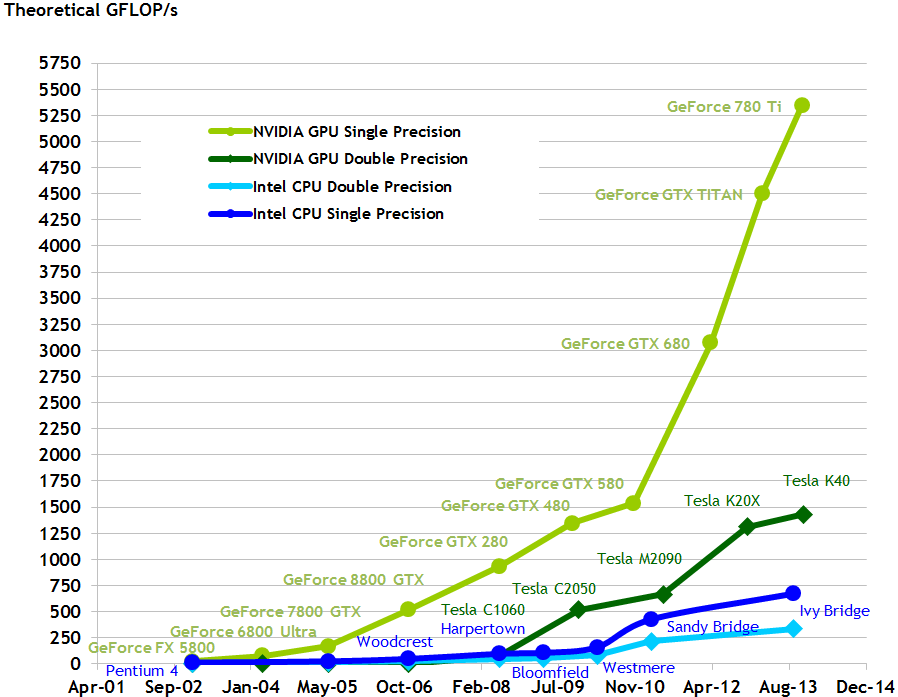
\includegraphics[width=10cm]{floating-point-operations-per-second.png}
    \caption{Theoretical throughput of some NVIDIA GPUs and Intel Processors, from\cite{cuda}. However the chart does not contain a Xeon Phi processor.}
    \label{fig:gpu_vs_cpu}
\end{figure}

\begin{figure}[h]
    \centering
    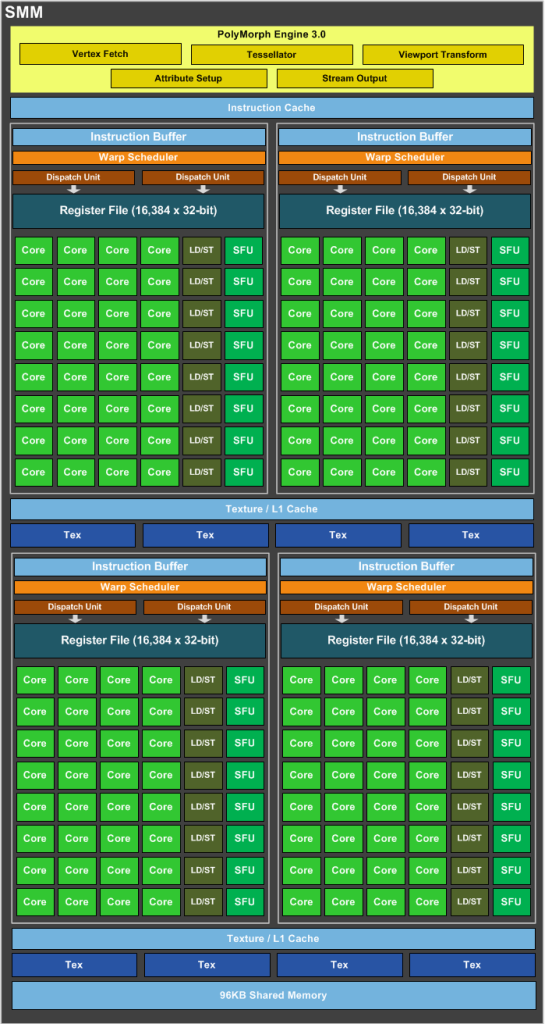
\includegraphics[width=11cm]{gpu_scheme.png}
    \caption{Layout of the Maxwell architecture, from \cite{nvidia_maxwell}}
    \label{fig:gpu_scheme}
\end{figure}

GPUs are made to process images in a fast manner so that games and similar tasks runs smoothly\cite{cuda}. Because GPUs are made for image processing they are GPUs have a large number of cores(~1000-2000)\cite{cuda, nvtesla}. Each core is slower than a core in a CPU, however the number of cores makes up for it. The downside is that it's slower than a normal CPU for sequential tasks so the program has to take advantage of the extreme parallelism to get good speed\cite{cuda_best_practice}. The memory of the GPU is separate from the computers main memory which means that the data needs to be transferred between the memories which increases the programs complexity\cite{cuda}.\\
\\
The GPU cores work in a manner that is similar to SIMD\cite{cuda}. The cores also have fewer optimizations than CPUs, this means that they can then devote a larger portion of the chip to the calculations as seen in figure \ref{fig:gpu_scheme}. For instance NVIDIAs GPUs lack optimizations such as branch prediction and speculative execution talked about in section \ref{optimizations} \cite{cuda}. Their caches are also much smaller than the CPUs\cite{cuda}. Another inheritance from the image processing is that they are much faster with single precision than with double precision data types\cite{cuda, nvtesla}. A CPU drops slightly in performance when using double precision however much less than a GPU as seen in figure \ref{fig:gpu_vs_cpu}. Single and double precision refers to how many bytes are used to store the decimal numbers, fewer bytes means less numerical precision.

\begin{figure}[h]
    \centering
    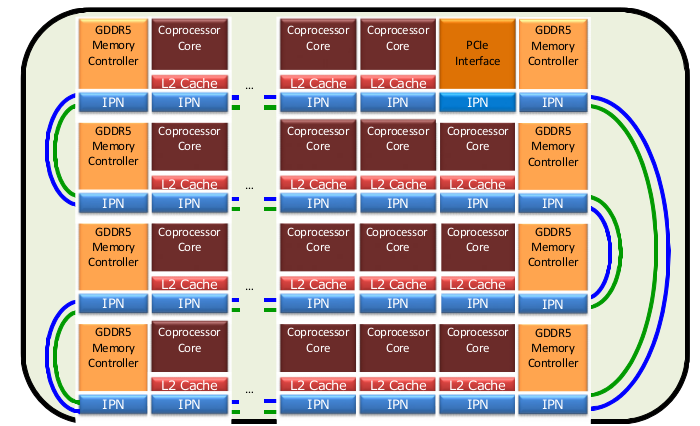
\includegraphics[width=12cm]{knigths_corner_silicon_layout.png}
    \caption{Knights Corner silicon layout, from\cite{intel_knights_corner}}
    \label{fig:knights_corner_layout}
\end{figure}

Intels answer to the increasing popularity of GPUs for general computing is Xeon Phi\cite{jeffers2013intel}. It has elements of GPU architecture however is still more like a CPU. It has separate memory and many cores(50+)\cite{jeffers2013intel}. It is MIMD which can be good for codes that diverge a lot, for ease of use however it has the possibly to use more SIMD like structures\cite{jeffers2013intel}. It is possible to only use the Xeon Phis memory and avoid the memory transfers that way. The memory is relatively small compared to the main memory so if the program needs a lot of memory transfers are likely needed. The cores of the Xeon Phi lacks some of the normal optimizations, e.g. out of order execution\cite{jeffers2013intel}.

\subsubsection{GPU vs Xeon Phi, Why use GPUs for Interaction?}
\label{gpu_gwas}
The choice depends largely on the algorithm, performance requirements, etc. For instance if the algorithm contains many points of divergence Xeon Phi is likely faster because Xeon Phi is MIMD while GPU is SIMT. That Xeon Phi is MIMD also means it can be applied to a broader set of problems\cite{jeffers2013intel}. A one on one comparison of speed might not the correct choice either because of the different prices of the hardware and power consumption. Speed per power consumption or price can be more relevant.\\
\\
GPUs are good for interaction algorithms because most methods consider each combination independently and in this case also that LR consists of linear algebra operations. Linear algebra with sufficiently large matrices and vectors suits well with the GPUs SIMT architecture\cite{cublas, cuda}. Several studies got high gains from implementing their algorithms on GPU\cite{gwis,gboost,gmdr_gpu,cuda_lr,genie_2012,plink_gpu}. However most studies had CPU versions that were not parallel so it is likely that the gains would have been less if they had compared to an optimized and parallel CPU version. One study made a comparison of their algorithm between using a CPU cluster and using a GPU\cite{jiang_accelerating}. They found that 16 CPU nodes had the same performance as a single GTX 280 card\cite{jiang_accelerating}.

%\subsection{Data Storage}
%TODO write about data storage

\subsection{Clusters}
%TODO fix cluster section
\label{clusers}

\begin{figure}[h]
    \centering
    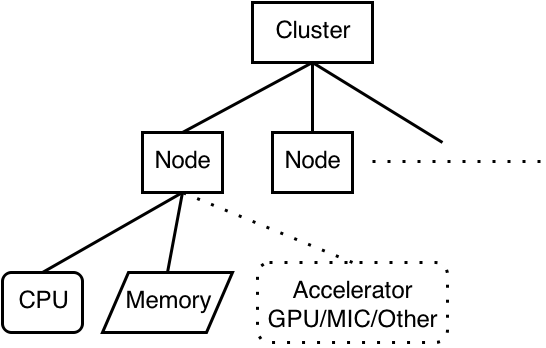
\includegraphics[width=10cm]{Cluster.png}
    \caption{Basic overview of a cluster}
    \label{fig:cluster}
\end{figure}

Clusters are collections of computers that can work together in several ways and are so tightly connected that they can usually be viewed as a single system. They communicate over a shared network but have separate memory and processors. Storage is usually shared. A computer in a cluster is called a \emph{node}. \cite{intro_hpc, introduction_hpc_hager}

%various programming models, shared memory and so on
%shared memory, cache coherrency and stuff

%mpi is commonly used for clusters\cite{introduction_hpc_hager}

%top 500\cite{TOP500}

%Few clusters used GPUs before 2009 but now mix of GPUs and CPUs are common among the top clusters. It was driven largely by demand for power saving while still giving high performance. The GPUs can do the heavy computation while other parts are used on CPU. \cite{introduction_hpc_hager}
%Something about Intel MIC

%Flops is not everything, bad performance compare to theoretical maximum
%Stuck in network, hard drives, etc. Latency
%Very few programs scale to the largest clusters

%\cite{introduction_hpc_hager}

\clearpage
\section{CUDA programming model}
\label{cuda_programming_model}
This section is about GPU programming in more detail using NVIDIAs CUDA(Compute Unified Device Architecture)\cite{cuda}. CUDA extends C and C++ with some additional functionality that can be used to perform operations on NVIDAs GPUs. It provides a separate compiler to compile the GPU code called nvcc\cite{cuda}. Different GPUs support different CUDA functions, each NVIDIA GPU has a value called computational capability. The higher the value the more features of CUDA are supported on that GPU. Some properties also vary between the different underlying architectures. This means that it is important to know what kind of capability the GPU to be used has so that the program does not need features that are not there. The things described here might not apply to GPUs with compute capability below 3. There are GPUs made specifically for calculations rather than games. This section is an summary of how CUDA works from the CUDA programming guide\cite{cuda} and CUDA best practices guide\cite{cuda_best_practice}.\\
\\
In CUDA the GPU is called \emph{device} and systems CPU and memory is the \emph{host}. To perform operations on the device a type of function called \emph{kernel} is used. A kernel is works mostly as a normal C/C++ function with the addition of some specifiers to provided options to set number of threads and so on. Example \ref{ex:simple_kernel_device} is an example of a simple kernel definition and example \ref{ex:simple_kernel_host} shows how it can be called from the host code. The kernel add each element of the arrays A and B storing it in C. Each thread performs on addition and knows why elements to use based on it's id. The call to the kernel is made by giving three arrays and the number of threads to be used as N. In this case N needs to be the length of the arrays.\\
\\
The \_\_global\_\_ keyword in front of the function declaration tells nvcc that it is a kernel. The $<<<N,M>>>$ specifier tells the compiler how many $N$ blocks and how many $M$ threads per block that the kernel should use\cite{cuda}. A block is a group of threads and shares some memory and resources. The blocks can be executed in any order so they need to be completely independent from each other but variables can be shared among threads inside a block\cite{cuda}. This allows the program to scale to different GPUs as shown in figure \ref{fig:blocks_scaling}. The blocks are  organized in a one, two or three dimensional \emph{grid}. These can be accessed by each thread so it knows which grid it is in as illustrated in figure \ref{fig:grid_2d}. This can be used to make it easier to assign the threads to the correct bit of the calculation. For instance using a two dimensional grid is good for matrices\cite{cuda, cuda_best_practice}.

\stepcounter{ExamplesCounter}
\begin{algorithm}
\DontPrintSemicolon
\SetStartEndCondition{ (}{)}{)}\SetAlgoBlockMarkers{\{}{\}}
\SetKwProg{Fn}{}{}{}\SetKwFunction{FRecurs}{void FnRecursive}
\SetKwFor{For}{for}{}{}
\SetKwIF{If}{ElseIf}{Else}{if}{}{elif}{else}{}
\SetKwFor{While}{while}{}{}
\SetKwRepeat{Repeat}{repeat}{until}
\AlgoDisplayBlockMarkers
\SetAlgoNoLine
\SetFuncSty{}
\SetArgSty{}

\SetAlgoRefName{\arabic{ExamplesCounter}}
\SetAlgorithmName{Example}{List of Examples}

\SetKwInOut{data}{Data}
\BlankLine \BlankLine

\data{Vectors \textit{A, B, C} as C-style arrays}

\BlankLine \BlankLine

\SetKwFunction{KwFn}{\textcolor{kernel}{\_\_global\_\_} void \KwSty{Add}}

\Fn(){\KwFn{\textcolor{keyword}{float}* $A$, \textcolor{keyword}{float}* $B$, \textcolor{keyword}{float}* $C$}}{
\textcolor{keyword}{int} $i$ = threadIdx.$x$;\;
$C[i]$ = $A[i]$ $+$ $B[i]$;\;
}

\caption{Example of a declaration of a simple kernel}
\example{Example of a declaration of a simple kernel}
\label{ex:simple_kernel_device}
\end{algorithm}

\stepcounter{ExamplesCounter}
\begin{algorithm}
\DontPrintSemicolon
\SetStartEndCondition{ (}{)}{)}\SetAlgoBlockMarkers{\{}{\}}%
\SetKwProg{Fn}{}{}{}\SetKwFunction{FRecurs}{void FnRecursive}%
\SetKwFor{For}{for}{}{}%
\SetKwIF{If}{ElseIf}{Else}{if}{}{elif}{else}{}%
\SetKwFor{While}{while}{}{}%
\SetKwRepeat{Repeat}{repeat}{until}%
\AlgoDisplayBlockMarkers\SetAlgoNoLine%

\SetAlgoRefName{\arabic{ExamplesCounter}}
\SetAlgorithmName{Example}{List of Examples}

\SetKwInOut{data}{Data}
\BlankLine \BlankLine

\data{Vectors \textit{A, B, C} of length $N$ as C-style arrays}

\BlankLine \BlankLine

\textbf{Add}\textcolor{kernel}{$<<<$1,$N>>>$}($A, B, C$);\;

\caption{Host code to call the kernel in example \ref{ex:simple_kernel_device} with $N$ threads}
\example{Host code to call the kernel in example \ref{ex:simple_kernel_device} with $N$ threads}
\label{ex:simple_kernel_host}
\end{algorithm}

\begin{figure}[h]
    \centering
    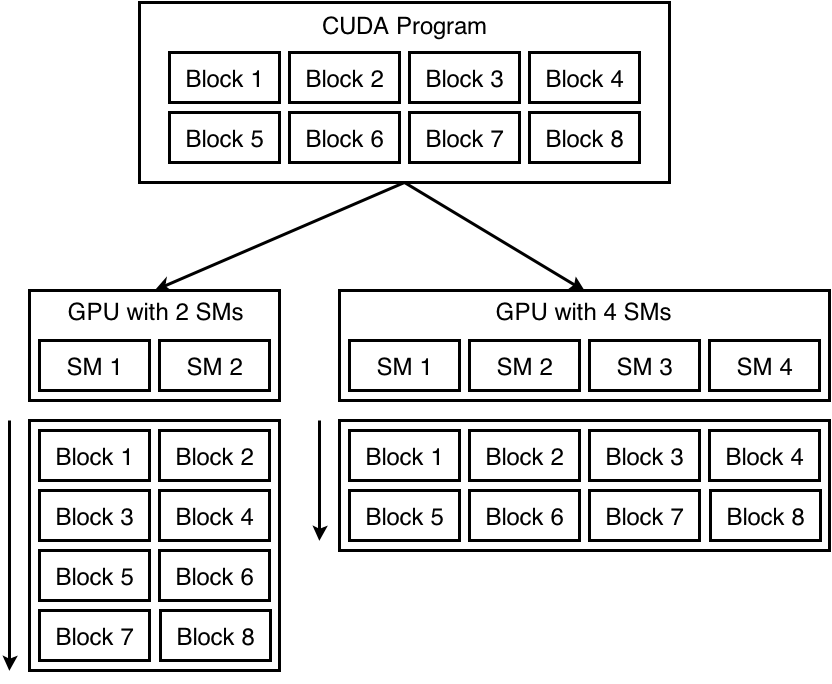
\includegraphics[width=10cm]{grid_scale.png}
    \caption{Blocks execution depending on the number of streaming multiprocessors}
    \label{fig:blocks_scaling}
\end{figure}

\begin{figure}[h]
    \centering
    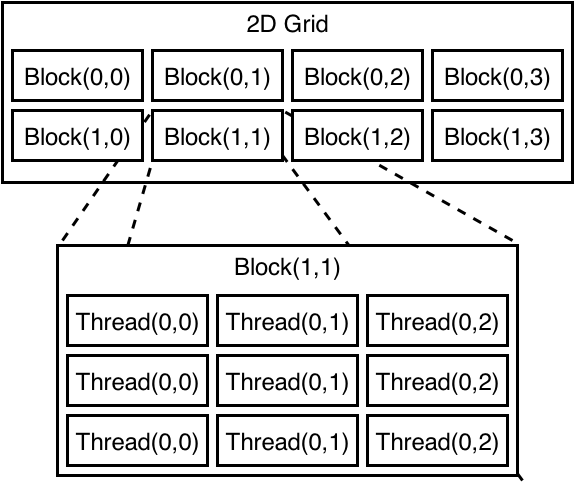
\includegraphics[width=8cm]{2D_grid.png}
    \caption{2D grid of blocks}
    \label{fig:grid_2d}
\end{figure}

\newpage

\begin{figure}[h]
    \centering
    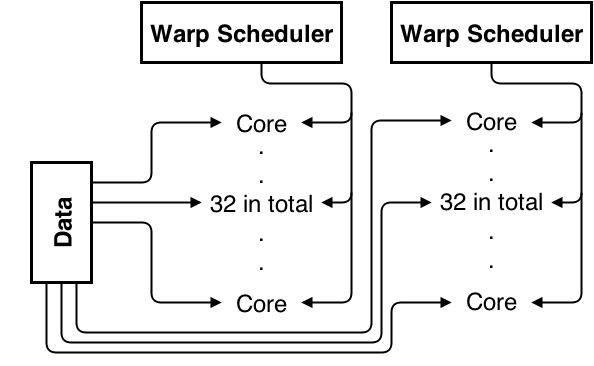
\includegraphics[width=8cm]{SIMT.png}
    \caption{SIMT architecture}
    \label{fig:SIMT}
\end{figure}

The streaming multiprocessors(SM) is the hardware that handles the execution of these blocks and can execute hundreds of threads concurrently. It uses \emph{SIMT}(Single-Instruction, Multiple-Thread) which is similar to SIMD described earlier in section \ref{concurrency}. SIMT works mostly as SIMD except that it can act as MIMD on collections of threads called \emph{warps}. Each warp consists of 32 threads. When an SM gets a block it is split into warps that are assigned to warp schedulers. Each warp scheduler gives one instruction to a warp so full efficiency is achieved when all the 32 threads perform the same instruction. If there is any divergence it has to disable unrelated threads, so divergence can be costly. However different groups of warps are on different warps schedulers so can diverge without problem.\cite{cuda}

\subsection{Device Memory}
The GPUs memory is physically on a different device separate from the computers main memory which means that they have separate memory spaces. An object in one memory is not accessible in the other memory. The computers main memory is the \emph{host memory} and the GPUs memory is the \emph{device memory}. Since they are separate data has to be transferred to the device memory and this is done by explicit calls to transfer sections of the hosts memory.\cite{cuda}\\
\\
The GPU also have several different types of memory\cite{cuda}. Correct usage can give increased speed\cite{cuda, cuda_best_practice}.

\begin{itemize}
  \item Register memory is located on the multiprocessor and usually costs zero cycles to access. The multiprocessor splits the available registers over its threads so if there are many threads that uses many variables not all of them will fit in the register. This is why a program sometimes can be faster with lower number of threads.\cite{cuda}
  \item Global memory is the main memory of the GPU and is accessible from all threads and blocks. However it is relatively slow to access.\cite{cuda}
  \item Shared memory is shared inside a block and is faster than global memory. However it is limited in size.\cite{cuda}
  \item Constant memory is small however it is read only which enables some optimizations. It is best used for small variables that all threads access.\cite{cuda}
  \item Local memory is tied to the threads scope, however it still resides off-chip so it has the same access time as global memory.\cite{cuda}
  \item Texture memory is read only and can be faster to access than global memory in some situations. This was more important in older GPUs when global memory was not cached.\cite{plink_gpu, cuda}
  \item Read-only cache is available on GPUs based on Kepler architecture and uses the same cache as the texture memory. The data as to be read only each multiprocessor can have up to 48kb of space depending on GPU.\cite{kepler_tuning_guide}
\end{itemize}

\subsection{Streams}
\label{streams}
The kernel calls can be made on a \emph{stream}. The easiest way to think of the stream is as queue. The kernels on a stream will be executed in the order they are made but kernels from different streams can be executed in any order given there is enough computational resources. In this way it is possible to execute up to 32 concurrent kernels depending on GPU.\cite{cuda}\\
\\
This is not entirely true for some GPU architectures because they only have one queue for the kernels. Because of this independent kernels from different streams can block each other. If we have a group of kernels and issue them on stream one first and then on stream two all the kernels in stream two will be stuck in the queue waiting for the kernels in stream one to finish. This is because the kernels queue only looks at the first kernels to see if they can be executed. The second kernel in the first stream then blocks the queue from moving forward so it will not see the kernels on stream two that could be executed. Newer architectures after Kepler on the other hand has several queues so they don't have this problem.\cite{cuda, cuda_best_practice, kepler_tuning_guide}\\
\\
Streams are also important for asynchronous transfers. These transfers are executed on a stream and just as kernels gets executed after the previous kernels on the same stream is done. The advantage is that other streams can do calculations as normal while the transfer happens. This can hide the time for transfers completely in some situations as shown in \ref{fig:ascynchronous}. However the host memory has to be pinned, pinned memory means that the operative system can not page that memory. Paging is that the operative system stores a part of the memory in another area, usually the disk memory, to save space in the memory. Too much pinned memory can slow down the computer.\cite{cuda, overlap_transfers_cuda}\\
\\
However there is problem that asynchronous transfers can cause depending on the GPUs architecture\cite{overlap_transfers_cuda, cuda_fortran_overlap}. Some older GPUs only have one copy engine while newer have one for each direction, one to the GPU and one from the GPU\cite{overlap_transfers_cuda, cuda_fortran_overlap}. This can affect how the calls should be ordered and using the wrong one can make the performance worse than without using asynchronous transfers\cite{overlap_transfers_cuda, cuda_fortran_overlap}.

There is an example of this in \cite{cuda_fortran_overlap} which illustrates the problem. They have four versions of the same code, a sequential transfer version and three asynchronous transfer versions. Two different GPUs were used, one had one copy engine the other had two. In the asynchronous the data is split over four streams coloured differently in the figure \ref{fig:ascynchronous}. Version 1 initiates the calls by looping over the streams one by one and doing the transfer and kernel calls on that stream before moving on to the next\cite{cuda_fortran_overlap}. Version 2 makes all the host to device transfer calls for all streams first, then the kernels and then the device to host transfer call\cite{cuda_fortran_overlap}. Version 3 is the same as version 2 but with a dummy even after each kernel\cite{cuda_fortran_overlap}. The figure \ref{fig:ascynchronous} shows how the transfers and kernels are executed on the GPU.

\begin{figure}[h]
    \centering
    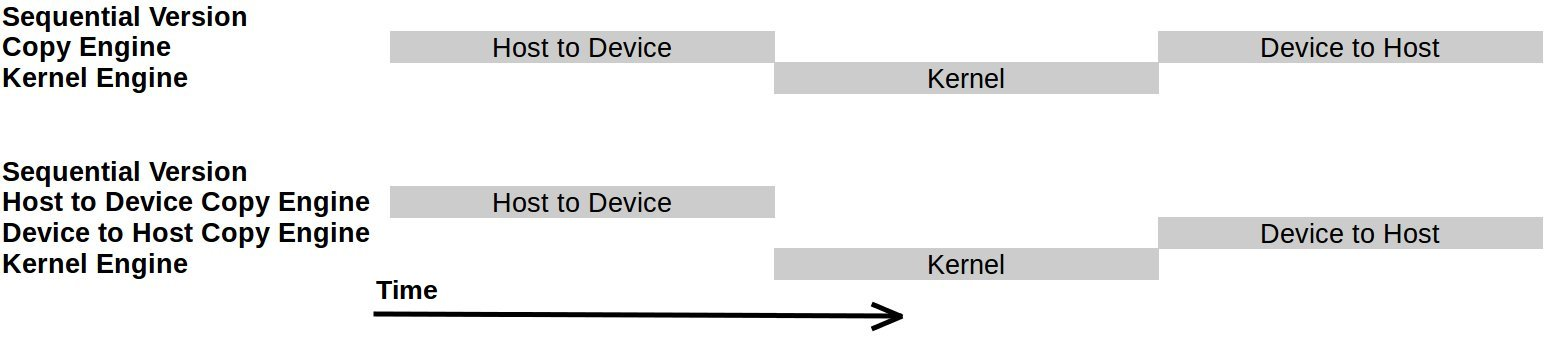
\includegraphics[width=12cm]{streams_seq.jpg}
    \caption{Sequential versions}
    \label{fig:sequential}
\end{figure}

\begin{figure}[h]
    \centering
    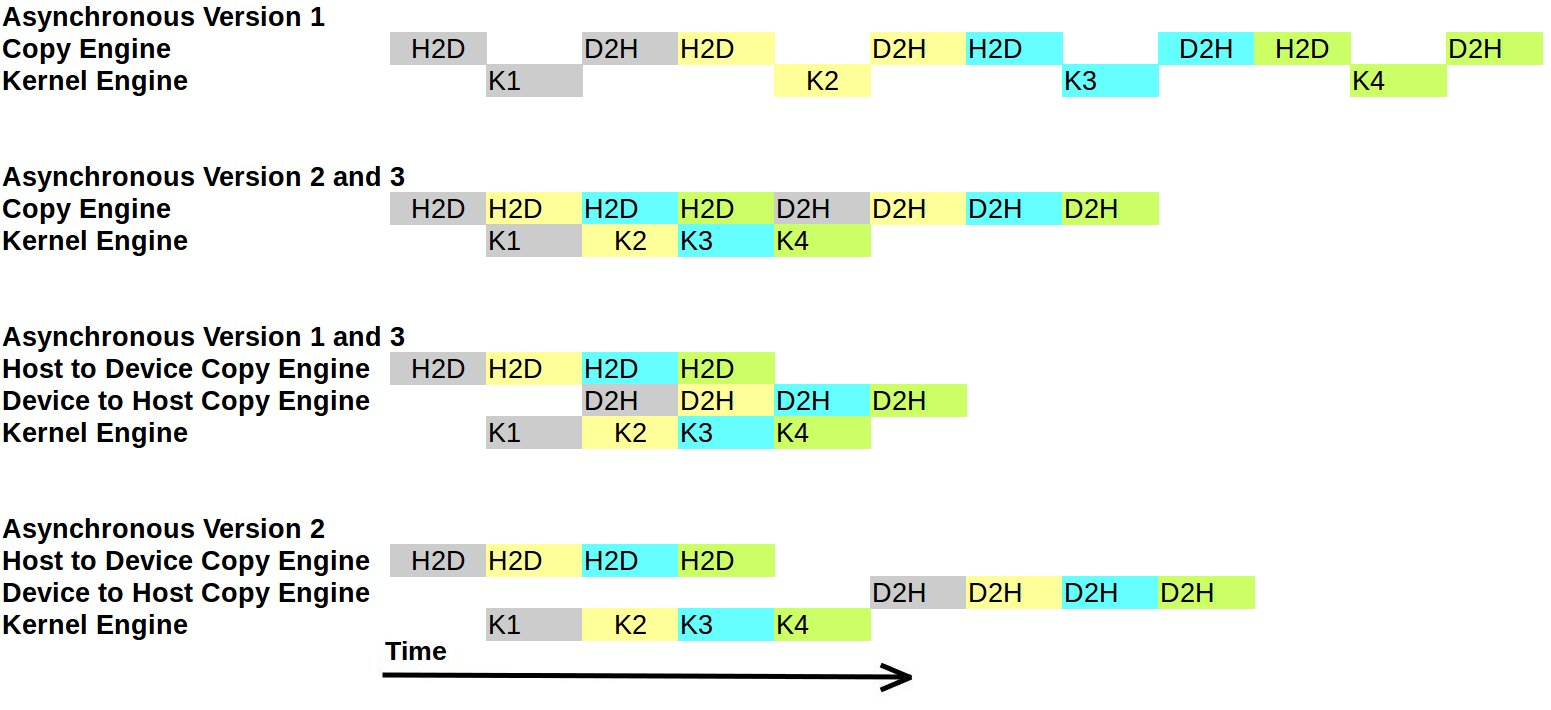
\includegraphics[width=12cm]{streams_async.jpg}
    \caption{Asynchronous versions. D2H=device to host transfer. H2D=host to device transfer. Each colour represents a stream.}
    \label{fig:ascynchronous}
\end{figure}

\subsection{Efficient CUDA}
One of the main criticism against GPUs for general computing purposes is that it is hard to get good performance because it requires good knowledge about details of the GPU architecture, especially the memory architecture. This section is a summary of things that can be good to consider for CUDA programs from the CUDA programming guide\cite{cuda}, CUDA best practices guide \cite{cuda_best_practice} and a similar list as this one, however slightly outdated now since it is from 2010, from a master thesis about GPU in GWAS\cite{plink_gpu}.
\\
\begin{description}
  \item[Maximize parallelism] \hfill \\
  Structure the program and the algorithm in such a way that it is as parallel as possible and overlap the serial parts on CPU with calculations on the GPU.\cite{plink_gpu, cuda}
  \item[Minimize transfers between host and device] \hfill \\
  Moving data between host and device is expensive and should be avoided if possible. It can be better to run serial parts on the GPU rather than moving the data to the host to do the calculation on the CPU. The bandwidth between host and device is one of the large performance bottlenecks. This can be a problem when the data is to large to fit in the relatively small GPU dram.\cite{cuda, cuda_best_practice}
  \item[Find the optimal number of blocks and threads] \hfill \\
  There are many things affected by the number of blocks and threads so they should be considered carefully. It is a good idea to parametrize them so that they can be changed for future hardware and varied for optimization. NVIDIA has an occupancy calculator which can be helpful in determining the optimal numbers, however high occupancy does not mean high performance.\cite{cuda, cuda_best_practice}\\
  \\
  The number of blocks should be larger than the number of multiprocessors so that all multiprocessors have at least one block to execute. Having two blocks or more per multiprocessor can be good so that there are blocks that aren't waiting for a \_\_syncthreads() that can be executed. However this is not always possible due to shared memory usage and similar.\cite{cuda_best_practice}\\
  \\  
  The number of threads per block should be a multiplier of 32 but minimum 64. It's also important to remember that multiple concurrent blocks can reside on the same multiprocessor. Too large number of threads in a block and parts of the multiprocessor might be idle since there aren't a block small enough to use those threads. Between 128 and 256 threads is a good place to start.\cite{cuda_best_practice}
  \item[Use streams and asynchronous transfers] \hfill \\
  By using streams it is possible to overlap memory transfers with calculations as mentioned before. This means that the data for the next batch can be transferred while the current batch is calculated and when it is done it can start calculating on the next batch directly after the current one is done. This can hide the time for transfers completely in some situations. Depending on the time the transfers take versus the time the calculations take this can give significant speedup.\cite{cuda, overlap_transfers_cuda, kepler_tuning_guide}
  \item[Use the correct memory type and caches] \hfill \\
  Correct use of caches and memory is important for both CPU\cite{drepper2007cpumemory} and GPU. However it is more complicated on GPU since the caches are smaller and there are several types of memory as mentioned before\cite{cuda, cuda_best_practice}.
  \item[Avoid divergence] \hfill \\
  Each thread in a warp executes the same instruction at the same time so if some of threads diverge the rest will be ideal until they are at the same instruction again. This means it is important to use control structures such as if statements carefully to prevent threads from idling.\cite{cuda, cuda_best_practice}
  \item[Avoid memory bank conflicts when using shared memory] \hfill \\
  Shared memory is divided into equally-sized memory modules called banks that can be accessed at the same time for higher bandwidth. Bank conflicts occur when separate threads access the same bank. On some GPUs it is fine if all threads access the same bank. Bank conflicts are split into as many conflict-free requests as needed.\cite{cuda, cuda_best_practice}
  \item[Use existing libraries] \hfill \\
  Instead of writing everything from scratch it is usually a good idea to use already existing libraries. Especially when performance is important and most task are non trivial on GPUs so using an already optimized library is a good idea. Some of the most popular libraries for CUDA are:
  \begin{itemize}
    \item CUBLAS: BLAS implementation for CUDA. BLAS and LAPACK is a standard for a library that provides highly optimized functions for linear algebra.\cite{cublas}
    \item CULAtools: BLAS and LAPACK implementation for CUDA for both dense and sparse matrices\cite{culatools}
    \item MAGMA: BLAS and LAPACK implementation among other things that can distribute the work on both CPU and GPU\cite{magma_2010}
    \item Thrust: Template based library that tries to emulate C++ standard library\cite{thrust_gpu}
  \end{itemize}
  \item[Avoid slow instructions] \hfill \\
  There are some instructions that can be slow and should be avoided if possible, for instance type conversion, integer division and modulo. If a function is called with a floating point number that might be used as a double and require a conversion. By putting an $f$ at the end of the number it is told to be single precision float, for instance 0.5f. In some cases it is possible to use bitwise operations instead which is faster.\cite{cuda, cuda_best_practice}
  \item[Restricted pointers can give increased performance] \hfill \\
  Aliasing can be a problem as mentioned earlier. By using the \_\_restrict\_\_ keyword on pointers the compiler can be told that no aliasing will occur, however it is up to the programmer to make sure that is the case or there might be unexpected results. Not using aliasing reduces the number of memory accesses the CPU needs to make. However it increases register pressure so it can have an negative effect on performance.\cite{cuda}
  \item[Use fast math functions if precision isn't needed] \hfill \\
  There are three versions of the math functions. The double precision version is func() while the single precision function is funcf(). There is third faster but less accurate version \_funcf(). The option -use\_fast\_math makes the compiler change all the funcf() to \_funcf().\cite{cuda_best_practice}
  \item[Instruction level parallelism can increase speed]\hfill \\
  Just as for CPUs the GPUs can take advantage of instruction level parallelism. By unrolling loops this can give 2x the speed relatively simple\cite{volkov2011unrolling}.
\end{description}

\clearpage
\section{Software Design}
How to design software so it can be maintained over time has been a problem for a long time. Object oriented languages such as C and later Java and C++ arose because of problems with maintaining software. Badly organized and written code will cost productivity in the future when bugs and other problems stack up because of earlier mistakes. Fixing those bugs are likely to time consuming because it can be hard to find where they originated from. All code gather problems overtime, however a well designed system will degenerate significantly slower than one that was designed carelessly. The code will also be read by ourselves and others later which means readability is important if a future reader is to understand the code and find the parts they are interested in. \cite{cleancode2008, design_patterns}\\
\\
This is also important in science where others might wish to use the tools or repeat the experiments. A recent study\cite{comp_repro_2013} found that the repeatability in computer science is low. They used the term reproducibility however repeatability is a more fitting term because they didn't try to reproduce the results from scratch, they tried to repeat it using the same code. Of 513 articles they received the code from 231, 108 failed to build, 21 failed to run properly\cite{comp_repro_2013}. The remaing 102 compiled and ran, however they did not check if the results of the program was correct\cite{comp_repro_2013}.\\
\\
There are ways to design the program and code in such a way that it is easier to read and maintain. Most of the things described here goes under the development technique called agile development and the concept of clean code and is a summary of some concepts from the book Clean Code\cite{cleancode2008}. SOLID is an acronym for five principles for object oriented programming and design\cite{cleancode2008}. When used together they are intended to make programs that are easy to maintain and extend\cite{cleancode2008}. As already mentioned readability is important. Correct names will make the code explain itself without other documentation, the code itself is the documentation\cite{cleancode2008}.

\begin{table}[h]
\begin{tabular}{ l l p{2in}}
  \hline
  Initial & Principal & Concept\\
  \hline
  S & Single responsibility principle & A class should only have a single responsibility \\
  O & Open/closed principle & A class should be open for extension but closed for modification \\
  L & Liskov substitution principle & If S is a subtype of T, then objects of type T may be replaced by objects of type S without without altering any of the desirable properties of the program(e.g. work performed)\\
  I & Interface segregation principle & Use several smaller and more specific interfaces instead of one large \\
  D & Dependency inversion principle & Depend on abstractions(e.g. interfaces) not details \\
  \hline  
\end{tabular}
\caption{The five SOLID principles, from \cite{cleancode2008}}
\label{table:solid_table}
\end{table}

Dependency injection is one way to implement dependency inversion principle\cite{cleancode2008}. Injection is passing the dependency to the dependent object. This is used instead of allowing the dependent object to construct or find the dependency.

\subsection{Unit Tests and Mocks}
\emph{Unit testing} involves testing the program in small units in isolation. Testing in isolation means that the test should only depend on the part of the program that is tested. If a part of the program is not working properly only its related tests should fail, not other tests for code that depends on it but otherwise works properly. This makes it easier to find errors when they do occur since the tests will pinpoint the unit which does not work. \emph{Integration testing} is used to test several units together to find possible errors  

%TODO integration tests

\cite{cleancode2008}\\
\\
It can be easy to denote test code as less important than the main code but they should be treated as equally important. Tests should also not be an inconvenience to use so they should be easy to run, take reasonable amount of time to complete and not require any outside interpretation whether they failed or not.\cite{cleancode2008}\\
\\
\emph{Mocking} is to replace a real object with a fake object called a \emph{mock} that for the code is indistinguishable from the real object. This allows one to create situations and test with more control and without depending on the real objects code. The second is important for unit tests since it enables one to test units that normally depend on others in isolation. In the first case it is useful in situations such as when one wants to test a class handling of a rare failure. Such failures can be hard and time consuming to induce. It is then easier to use a mock object that behaves like the failure has occurred. However mocking requires that the code for the class doesn't create the object itself since there is no way to replace the object with the mock. This is one of the reasons why dependency injection should be use.\cite{cleancode2008}

\subsection{Design Patterns}
\label{design_pattern}
A \emph{design pattern} in software design is a reusable general solution to a common recurring problem in a given context. It is templates and structures to solve the problem, however it is not code. However they are partially dependent on the programming language since different languages have different features and limitations.\cite{design_patterns}\\
\\
\emph{Consumer producer} is a concurrency pattern for when there are a number of consumers/workers and producers. They share a common queue for products. The producer generates some product and put it into the queue, while the the consumers consume the products. The problem is that the producers should not add to an non empty slot and that each product should only be consumed once.\cite{cleancode2008, design_patterns}\\
\\
%TODO builder pattern
Configuration pattern classes are used to reduce the number of parameters to functions. Instead of having a number of parameters to a function the parameters are put in a Configuration class. The Configuration class has two functions for each parameter, a \textbf{set} function and a \textbf{get} function. The \textbf{set} is used to set the parameter while \textbf{get} is used to get the parameter.\\
\\
%TODO adapter pattern
%TODO factories Factories allow the a class to delegate the construction 

\subsection{Version Control Software}
Backups for data, code, text and so on is important if something happens. One way to backup text and code projects is to use a version control software and is usually an important tool in developing\cite{git_book}. For this project Git was used and the source code can be found at \url{https://github.com/Berjiz/CuEira}. Version control software allows several developers to share a common \emph{repository} which allows them to work on different parts at the same time, it could even be in the same file\cite{git_book}. However changes at the same place causes \emph{merge conflicts} which usually needs to be solved manually\cite{git_book}. A version control software keeps track of all the changes made so if a part later turns out to be wrong that part can reverted to an older correct version\cite{git_book}. Version control software also have many other features\cite{git_book}.

\clearpage
\section{Performance Measures}
An important part in creating fast and efficient programs is to know how fast the program is under certain conditions and which parts of the program are slow\cite{introduction_hpc_hager}. For instance the speed could suddenly drop when too many threads, there might be a bottleneck in the communication, and so on.\\
\\
There are two ways to measure how long a program takes to execute\cite{introduction_hpc_hager}. Wall clock time is how long real life time the program took. The other is to measure the number of processor cycles spent. A parallel program will have shorter execution time than it is serial version however it will likely have spent more processor cycles due to overhead from communication and initialization of the threads. These two measures are useful for different kinds of comparisons. Wall clock time is better for overall performance while number of cycles is useful for comparing different algorithms\cite{introduction_hpc_hager, cuda_best_practice}.\\
\\
Speed up is a measure of how much faster then program is with a certain number of threads compared to the serial version. It's defined as\cite{introduction_hpc_hager}
$$S(p)=\frac{T(1)}{T(p)}$$
Where $T(1)$ is execution time of serial program and $T(p)$ is execution time of parallel program with p threads. Linear speedup is when S(p)=p\cite{introduction_hpc_hager}.\\
\\
Efficiency reflects how efficient the program is using p threads. Linear speed has efficiency 1. It's defined as\cite{introduction_hpc_hager}
$$E(p)=\frac{S(p)}{p}=\frac{T(1)}{pT(p)}$$
\\
Strong scaling refers to how the program handles a fixed problem size and increased number of processors\cite{introduction_hpc_hager}. An program with strong scaling has linear speedup\cite{introduction_hpc_hager}. Weak scaling refers to the execution time of the program when there is a fixed problem size \emph{per processor} and the number of processors is increased\cite{introduction_hpc_hager, cuda_best_practice}.\\
\\
It can be a good idea to plot these measures while varying p, this can show when a bottleneck occurs. Looking at the measures at node level can also be useful to get an idea of how increased number of nodes and therefore increased communication over the network affects the performance.

\newpage
\subsection{Amdahl's Law and Gustafson's Law}
Amdahl's Law is used to find the expected speedup of a system when parts of it are made concurrent. Simply it says that as the number of processors increases the parts that aren't parallel will start taking up more and more of the wall clock time and that the speedup for adding more processors will decrease as more and more processors are added and more time is spent relatively on the non parallel parts\cite{introduction_hpc_hager}. It's closely related to strong scaling.\cite{cuda_best_practice,2010_reevaluating_amdahl}\\
\\
It says that the expected speedup with F fraction of the code parallel and p threads is\cite{introduction_hpc_hager} 
$$S(p)=\frac{1}{(1-F)+\frac{F}{p}(1-F)}$$
As the number of threads grow towards infinity $S(p)$ converges on $\frac{1}{1-F}$. If we have 90\% of a code parallel then even with infinite number of threads we won't get a better speedup than ten.\cite{2010_reevaluating_amdahl}

\begin{figure}[h]
    \centering
    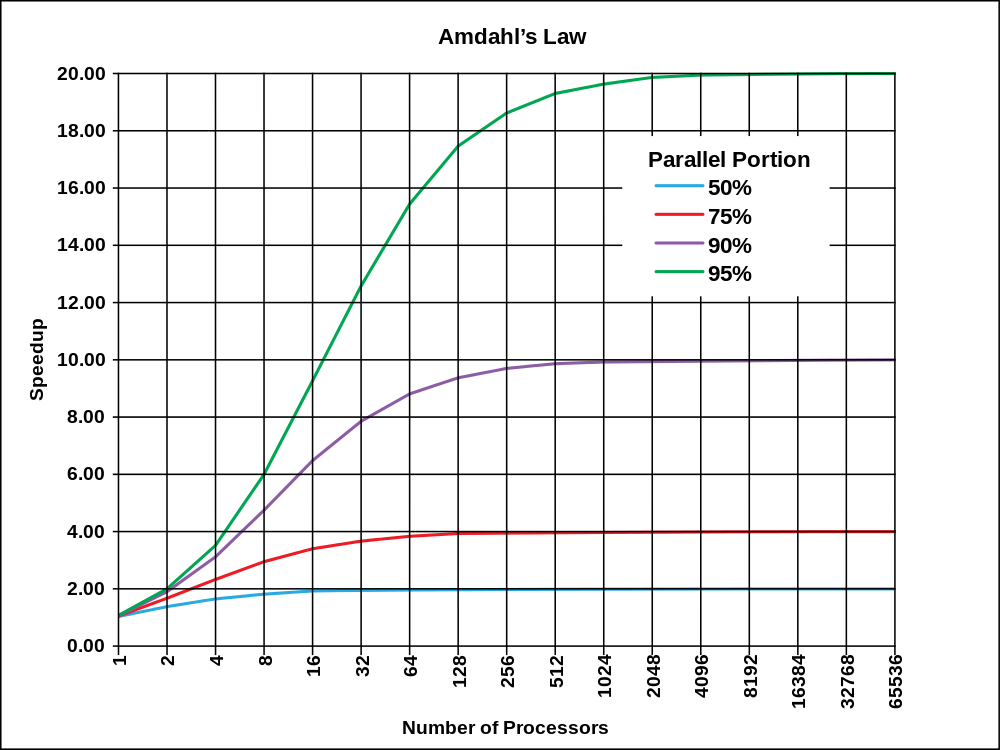
\includegraphics[width=11cm]{AmdahlsLaw.png}
    \caption{Illustration of Amdahl's Law. Wikipedia Commons}
    \label{fig:AmdahlsLaw}
\end{figure}

There are limitation to Amdahl's Law since it makes a couple of assumptions.

\begin{itemize}
  \item The number of executing threads remain constant over the course of the program.
  \item The parallel portion has perfect speedup. Often not true due to shared resources,eg caches, memory bandwidth, and shared data.
  \item The parallel portion has infinite scaling, not true due to similar limits as above. More threads will not increase performance after a while or might even decrease it.
  \item There is no overhead for creation and destruction of threads.
  \item The length of the serial portion is independent of the number of threads. Often the serial work is to divided the work to the threads, this work will obviously increase as the number of threads go up. More threads can also lead to more communication overhead.
  \item The serial portion can't be overlapped by the parallel parts. For instance with producer consumer type pattern the consumer could be strictly serial but the time it takes could be overlapped by the parallel producers.
\end{itemize}

This means it is most accurate with programs that are of the fork-join type, e.g. both serial and parallel parts\cite{gustafson1988reevaluating}.\\
\\
Gustafson's Law is closely related to Amdahl's Law and can in some ways be more accurate than Amdahl's Law\cite{gustafson1988reevaluating}. Gustafson's Law makes similar assumptions as Amdahl's Law however it also makes two additional statements. It states that problems tends to expand when provided with more computational power, e.g. increased precision by reducing grid size for simulations, higher frame rate for graphics and so on\cite{gustafson1988reevaluating, introduction_hpc_hager}. The second is that the parallel portion of the program tends to expand faster than the serial part, e.g. for matrix multiplication the initialization scales linearly with the matrix size while the multiplication itself scales as $O(n^3)$\cite{gustafson1988reevaluating, introduction_hpc_hager}. The former means that it is closely related to weak scaling\cite{introduction_hpc_hager}. So in a way it says that the execution time remains constant rather than the amount of data. More precise it says that the expected speedup with p threads and F fraction of the code that is parallel is\cite{gustafson1988reevaluating, cuda_best_practice, introduction_hpc_hager}
$$S(p)=p+(1-F)(1-p)$$

\begin{figure}[h]
    \centering
    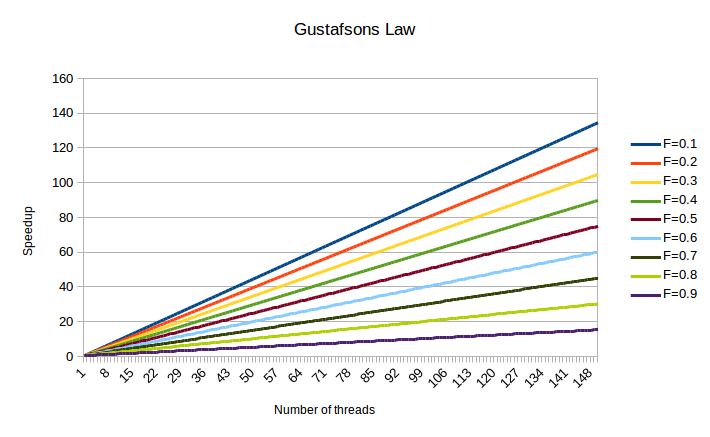
\includegraphics[width=13cm]{GustafsonsLaw.png}
    \caption{Illustration of Gustafson's Law}
    \label{fig:GustafsonsLaw}
\end{figure}

\subsection{Profilers}
There are applications called profilers that are made to assess the programs performance and resource consumption. They calculate some of the measures mentioned earlier and they also check hardware usage and how much time the program spends at various parts of the program. This is very useful for finding bottlenecks and other problems in the program. It does not matter if the algorithm is super fast if all the data is stuck in network transfers. The profilers can be hardware dependent so the manufactures usually provided them for their products.\cite{introduction_hpc_hager, cuda_best_practice}\\
\\
Nsight\cite{nvidia_nsight} is a combined profiler and integrated development environment(IDE) based on either Visual Studio or Eclipse. For this thesis Nsight Eclipse edition was used. It works as the usual Eclipse but has added functionality for CUDA and CUDA profiling\cite{nvidia_nsight}.

\begin{figure}[h]
    \centering
    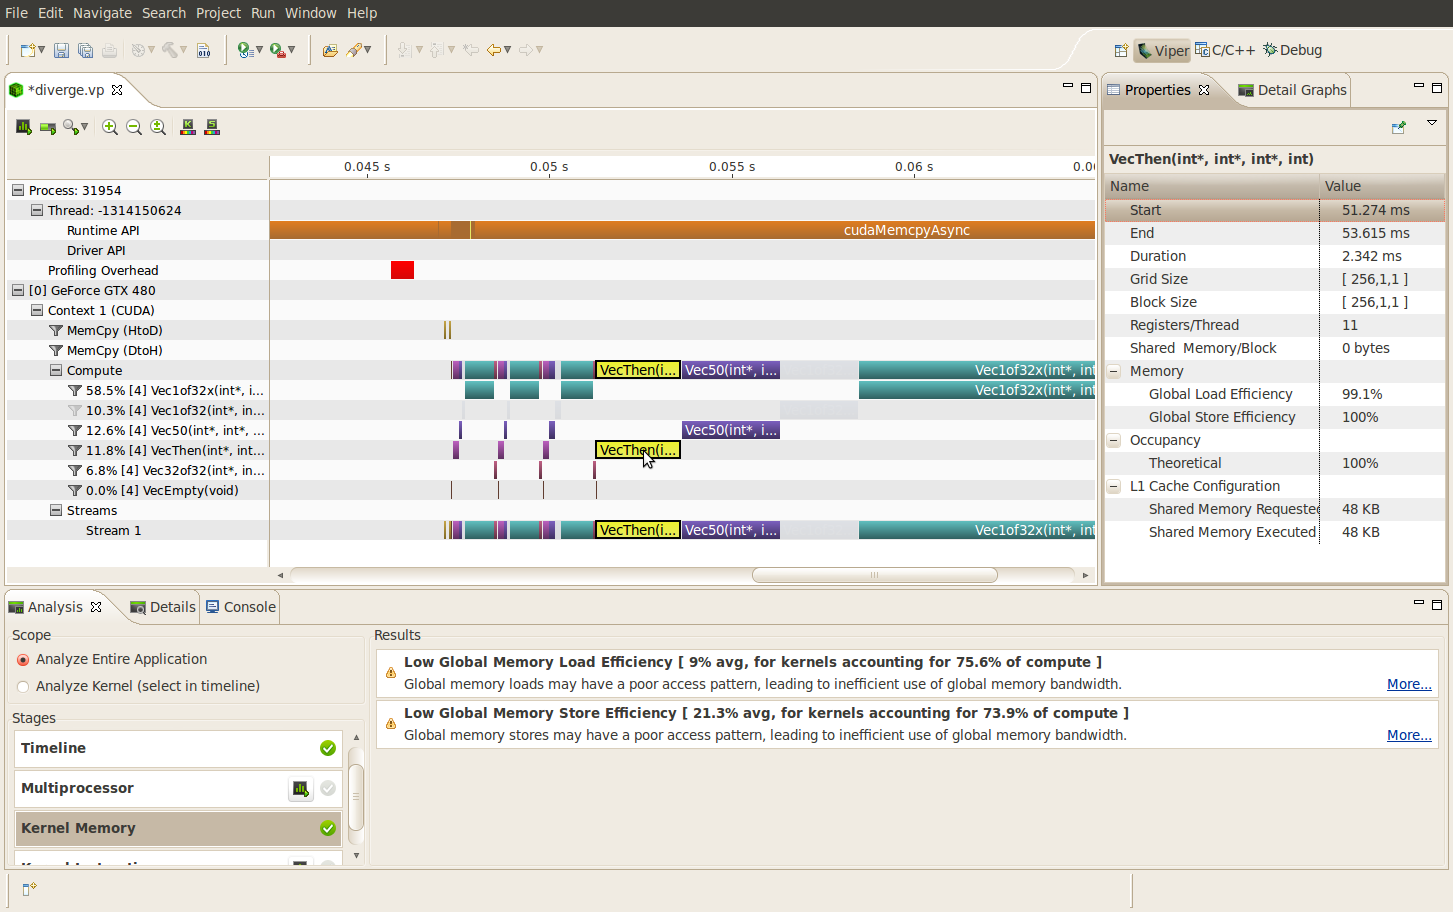
\includegraphics[width=10cm]{nsight_profiler.png}
    \caption{Screenshot of Nsight Eclipse Editions profiling section, from \cite{nvidia_nsight}}
    \label{fig:nsight_profiler}
\end{figure}

\newpage
\section{Algorithms}
\label{algorithm_background}
There are many algorithms and programs proposed for searching for interaction, most have focused on gene-gene interaction as already mentioned\cite{gene_enviroment_2013}. One of the challenges of gene-environment interaction is that environmental factors can be of any variable type(i.e. binary, continuous, categorical) which creates problems in various ways\cite{gene_enviroment_2013}. Gene-gene interaction tools can sometimes be used to find gene-environment interaction, however they usually require the variables to be binary or have other problems since they weren't designed for environmental interaction\cite{gene_enviroment_2013}.\\
\\
Both groups of computers(i.e. clusters) using regular processors\cite{biforce} and graphic processors\cite{gwis,gboost,gmdr_gpu,cuda_lr,genie_2012,plink_gpu} have been used for GWAS. Graphic processors for computing have become more popular in the last ten years. They have been a popular choice for some GWAS methods because each combination of variables can commonly be considered independently from the others. More about graphic processors in section \ref{gpu} and why the are good for GWAS in section \ref{gpu_gwas}.\\
\\
The methods can be roughly classified into four categories, exhaustive, stochastic, machine learning/data mining and stepwise\cite{fast_high_order_cluster}.\\
\\
\emph{Exhaustive search} is the most direct approach, it compares all combinations of the SNPs in the dataset. Exhaustive search methods will not miss a significant combination because it didn't consider that specific combination. However it also means that they can be slow since they will spend time on combinations other methods would skip completely. Multifactor-Dimensionality Reduction(MDR)\cite{mdr_2001} and BOOST\cite{boost_gene_gene} are two examples of this type of algorithm.\\
\\
\emph{Stochastic} methods uses random sampling to iterate through the data. BEAM\cite{beam_2007} is one example and it uses Markov Chain Monte Carlo(MCMC) method.\\
\\
\emph{Data Mining} and \emph{Machine Learning} are methods that try to learn patterns from data and tries to generalize it. MDR\cite{mdr_2001} is a type of data mining method and is among the most common methods used in GWAS. See section \ref{data_machine_learning} for more details.\\
\\
\emph{Stepwise} methods uses a filtering stage and a search stage. At the filtering stage uninteresting combinations are filtered out by using some exhaustive method. The other SNPs are the examined more carefully in the search stage. BOOST\cite{boost_gene_gene} is an example which uses succinct data structures and a likelihood ratio test to filter the data before applying log-linear models.

\newpage
\subsection{Logistic Regression}
\label{logistic_regression}
One way to model the contingency tables is by using \emph{logistic regression}. Logistic regression is a type of linear regression model for classification that models a latent probability for the outcomes. The outcomes are binary, however the method can be extended to multiple outcomes. In this work we will only consider them as binary. Logistic regression transforms the probability by using the \emph{logit} transformation. The logit transformation with probability $\pi$ is \cite{agresti_categorical}

\begin{equation}\label{eq:logit}
\log(\frac{\pi}{1-\pi})
\end{equation}

\begin{figure}[h]
    \centering
    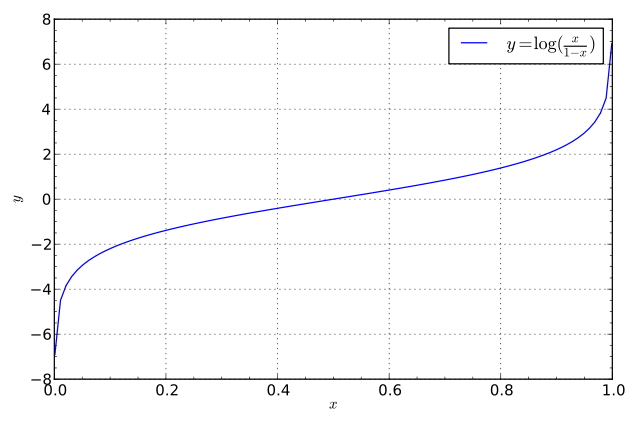
\includegraphics[width=10cm]{logit.png}
    \caption{Graph of the logit transformation. Wikipedia Commons}
    \label{fig:logit}
\end{figure}

The probability with a set of predictor variables \emph{X} is $\pi(X)=P(Y=1)$. The linear regression model with n predictors $X=(x_1,x_2,....,x_n)$, coefficients $\beta=(\beta_1, \beta_2,....,\beta_n)$ and by using the logit transformation is then\cite{agresti_categorical}
\begin{equation}\label{eq:logit_lr}
logit[\pi(X)]=\alpha+\beta X
\end{equation}

By moving the logit to the right side of the equation we get the model of the probability\cite{agresti_categorical}
\begin{equation}
\pi(X)=\frac{e^{\alpha+\beta X}}{1+e^{\alpha+\beta X}}
\end{equation}

The logit, equation \ref{eq:logit}, also happens to be the log of the odds(equation \ref{eq:odds})\cite{agresti_categorical}. By exponentiating both sides of equation \ref{eq:logit_lr} it shows that the odds is \cite{agresti_categorical}

\begin{equation}
e^{logit[\pi(X)]}=\frac{\pi(X)}{1-\pi(X)}=e^{\alpha+\beta X}=\Omega
\end{equation}

This means that $\exp{\beta}$ is the odds ratio since the odds increase by $\exp{\beta}$ for each unit increase of $X$\cite{agresti_categorical}. It can also been seen by taking the ratio of the odds using equation \ref{eq:odds_ratio} and  with $X=x+1$ and $X=x$

\begin{equation}
\theta=\frac{e^{\alpha+\beta (x+1)}}{e^{\alpha+\beta x}}=e^{\alpha+\beta (x+1)-\alpha-\beta x}=e^{\beta}
\end{equation}

Finding the $\beta$ coefficients are done in a similar way as with other linear regression models since they all are generalized linear models \cite{agresti_categorical}. It's usually done using  maximum likelihood(ML), via Newtons method\cite{agresti_categorical, uvehag_master_thesis}. It's an iterative method which means it can be relatively slow compared to non iterative methods. The pseudo code for the algorithm using Newtons method can be found in algorithm \ref{alg:lr} \cite{uvehag_master_thesis}. Line 13 is sometimes inside the loop, however since it is not needed for the actual iteration calculating it for every loop wastes time.

\begin{algorithm}
\DontPrintSemicolon
\SetKwInOut{data}{Data}
\BlankLine \BlankLine
\SetKwInOut{note}{Note}
\LinesNumbered

\data{$N$ number of data points\\
$M$ number of variables, excluding the intercept\\
$\boldsymbol{X}$ is an $N \times M$ matrix that contains the variables\\
$\boldsymbol{Y}$ is the outcomes with length $N$\\
$\beta$ has length $M$ and contains the initial values of $\beta$}

\note{$*$ is element by element multiplication}

\BlankLine \BlankLine
$\boldsymbol{X}\longleftarrow
\begin{pmatrix}
\begin{matrix}
  1\\
  \vdots\\
  1
\end{matrix} & \boldsymbol{X}
\end{pmatrix}
$\;

\BlankLine \BlankLine
$\beta\longleftarrow
\begin{pmatrix}
  0\\
  \beta
\end{pmatrix}
$\;

\BlankLine \BlankLine
$iter\longleftarrow 0$\;
$diff\longleftarrow 1$\;

\BlankLine \BlankLine
\While{$iter < max\_iter \; \boldsymbol{and} \; diff > threshold$}{
  $\beta_{old}\longleftarrow\beta$\;
  $p\longleftarrow \frac{e^{\boldsymbol{X} \cdot \beta}}{1+e^{\boldsymbol{X} \cdot \beta}}$\;
  $s\longleftarrow \boldsymbol{X^T}\cdot (\boldsymbol{Y}-p)$\;
  $\boldsymbol{J}\longleftarrow (\boldsymbol{X^T}\cdot (p*(1-p)))\cdot \boldsymbol{X}$\;
  $\beta\longleftarrow \beta_{old}+\boldsymbol{J}^{-1} \cdot s$\;
  $diff\longleftarrow \sum |\beta-\beta_{old}|$\;
  $iter\longleftarrow iter+1$\;
}
\BlankLine \BlankLine
$log \; likelihood\longleftarrow \sum (\boldsymbol{Y}*ln p+(1-\boldsymbol{Y})*ln(1-p))$\;

\caption{Logistic regression using maximum likelihood and Newtons method}
\algorithmslist{Logistic regression using maximum likelihood and Newtons method}
\label{alg:lr}
\end{algorithm}

\newpage
\newpage
\subsubsection{Matrix Inverse and Matrix Decomposition}
\label{matrix_inverse}
The inverse of the \emph{information matrix}, \textbf{J}, on line 10 in algorithm \ref{alg:lr} is generally not possible to do with normal matrix inversion because it is not defined for a general matrix\cite{albert1972regression}. However the \emph{pseudoinverse} is defined for a general matrix, it is denoted as $A^+$ for the matrix $A$\cite{albert1972regression, golub1970singular}. There are several types of pseudoinverse, one of the more common is the \emph{Moore-Penrose pseudoinverse} where $A^+$ is the matrix that satisfies equations \ref{eq:pseudo_1} to \ref{eq:pseudo_4}\cite{albert1972regression}.

\begin{equation}\label{eq:pseudo_1}
AA^+A=A
\end{equation}

\begin{equation}\label{eq:pseudo_2}
A^+AA^+=A^+
\end{equation}

\begin{equation}\label{eq:pseudo_3}
(AA^+)^T=AA^+
\end{equation}

\begin{equation}\label{eq:pseudo_4}
(A^+A)^T=A^+A
\end{equation}

\emph{Matrix decomposition}, also called \emph{matrix factorisation}, are methods to factorize a matrix into products of matrices\cite{golub1970singular}. Some of the decomposition methods can be used to find the pseudoinverse. \emph{Singular value decomposition}(SVD) is one of them and works for general matrices\cite{golub1970singular}. It's factorization of a  $n \times m$ matrix $A$ is shown in equation \ref{eq:svd}\cite{golub1970singular}.

\begin{equation}\label{eq:svd}
A=U \Sigma V^T
\end{equation}

Where $\Sigma$ is a diagonal matrix with non negative numbers, its diagonal values are the \emph{singular values} of $A$\cite{golub1970singular}. Using SVD the pseudoinverse is shown in equation \ref{eq:pseudo_svd}\cite{golub1970singular}. $\Sigma^+$ is the pseudoinverse of $\Sigma$. This is done by inverting each non zero element of the diagonal and transposing the matrix\cite{golub1970singular}.

\begin{equation}\label{eq:pseudo_svd}
A^+=V \Sigma^+ U^T
\end{equation}

\subsection{Data Mining and Machine Learning Approaches}
\label{data_machine_learning}
Approaches based on Data Mining and Machine Learning have been a popular choice for GWAS. MDR\cite{mdr_2001} and Random Forest(RF)\cite{random_forest} are among the most common ones\cite{gene_enviroment_2013,cordell_detect_review}. There are other methods as well such as clustering approaches \cite{fast_high_order_cluster}. Most of them are used for screening the data for possible interactions\cite{gene_enviroment_2013,cordell_detect_review}.\\
\\
Their biggest advantage is that they are usually non-parametric and designed with high dimensional data in mind. However they are prone to overfitting and the usual way to try to prevent that is to use cross validation and sometimes permutation tests. It means that even if the method itself is fast it is repeated so many times that the whole algorithm can be slow in the end.\cite{cordell_detect_review}

\subsubsection{Multifactor-Dimensionality Reduction}
MDR is a method that reduces the number of dimensions(i.e. variable) by combining several dimensions into one. In GWAS it combines the variables that are suspected to interact. This new variable is then compared against the outcome. If the new variables predictability of the outcome is high enough then the variables that were combined are considered to interact. This process is usually repeated on all pair combinations of variables.\\
\\
The reduction from $n$ dimensions is done by calculating the ratio of cases versus controls for each combination of the possible values of the variables. If the ratio is above a certain threshold all the members of that groups get the value 1 for the new dimension, otherwise 0. Accuracy of the model is done by using cross validation and permutation tests, in simpler words it means that it reshuffles the data randomly and recalculates the model many times to get an estimate of the models certainty. Because of that MDR can be slow. However it is still usually faster than exhaustive search with regression methods.\cite{cordell_detect_review,mdr_2001}\\
\\
MDR can been used for gene-environment interaction but requires modifications since MDR can only handle binary variables. There are extensions that can use continues variables, however these are regression based so these will be slower than regular MDR.\cite{gene_enviroment_2013}\\
\\
A simple example of MDR using exclusive or (XOR). XOR is an logical operator that is true if one and only one of its two variables is true. We have 4 possible combinations and an occurrence for each of them, see table \ref{table:xor_table}. The combination (1,0) and (0,1) both have one case with outcome 1 so MDR will classify them as 1 in the new variable Z, the other two combinations have outcome 0 so will be classified with Z=0, see table \ref{table:xor_mdr_table}. From here it is easy to make an predictor from Z to the outcome Y by comparing the values.

\begin{table}[h]
\begin{tabular}{ | c | c | c | }
  \hline
  \textbf{Y} & $\mathbf{X_1}$ & $\mathbf{X_2}$ \\
  \hline
  1 & 1 & 0 \\
  \hline 
  1 & 0 & 1 \\
  \hline
  0 & 0 & 0 \\
  \hline
  0 & 1 & 1 \\
  \hline
\end{tabular}
\caption{XOR table with outcome $\mathbf{Y}$ and variables $\mathbf{X_1}$ and $\mathbf{X_2}$.}
\label{table:xor_table}
\end{table}

\begin{table}[h]
\begin{tabular}{ | c | c | }
  \hline
  \textbf{Y} & \textbf{Z} \\
  \hline
  1 & 1 \\
  \hline
  1 & 1 \\
  \hline
  0 & 0 \\
  \hline
  0 & 0 \\
  \hline
\end{tabular}
\caption{XOR table with $\mathbf{X_1}$ and $\mathbf{X_2}$ combined into $\mathbf{Z}$ using MDR.}
\label{table:xor_mdr_table}
\end{table}

\subsubsection{Random Forest}
RF is an ensemble learning method\cite{random_forest}. Ensemble methods combine multiple models to improve performance. RF takes randomized samples of the data and builds decision trees on each of them. These trees are then combined to form the classifier. Usually hundreds or thousands of trees are used depending on the problem\cite{random_forest}. One of the most popular variants of Random Forest for GWAS is Random Jungle\cite{random_jungle}.\\
\\
It has been shown in high dimensional data that RF tends to only rank interacting factors high if they have strong marginal effects\cite{winham_rf_2012}. Also the ranking of the variables does not indicate which factor it is interacting with either since it is based on the joint distributions\cite{gene_enviroment_2013}. How to incorporate the environmental factors in RF is also not obvious and using variables with very different scales can bias the results\cite{gene_enviroment_2013}.

\begin{figure}[h]
    \centering
    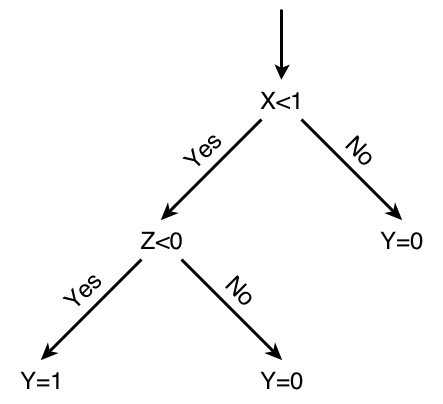
\includegraphics[width=7cm]{Decision_Tree.png}
    \caption{A example of a decision tree}
    \label{fig:DecisionTree}
\end{figure}

\newpage
\chapter{Implementation}
\label{implementation}
This section will explain the implementation of the program starting with a short summary of how JEIRA and GEISA works. After that is a more thorough look at the structure and implementation of CuEira.\\
\\
The input files for all these programs are PLINK data files. However CuEira can only read the PLINK files in binary format. They also read a separate tab delimited file that contains the environmental data and covariates if any. For CuEira the covariates and environmental data is split in two files.

%\section{Terminology}
%\label{basic_program_term}
%TODO write about inheritance, namespaces, pointers, memory, enums, exceptions

%An enum is a data type consisting of a set of named values. This is useful when the variable has a distinct set of values that makes more sense as text rather than something else. For instance gender can be stored as enum with the two values MALE and FEMALE, the enum values are commonly write in capital letters. The gender could be stored an int, however it is easier to understand the meaning of MALE than just a number and it also avoids potential errors with incorrect values. An enum can only have one of it's possible values while an int is not restricted in the same way.

\section{JEIRA and GEISA}
The descriptions and structures in this section applies to both JEIRA and GEISA since their underlying structure is the same, however the focus is on GEISA. They are written in Java and uses Javas built-in functions for concurrency.\\
\\
GEISA has three dependencies, two are provided as JAR files in the distribution so the user doesn't need to get them. Maven is only needed if the user wants to compile the program from the source.

\begin{description}
  \item[Apache Commons CLI] \hfill \\
  Provides command line interface, e.g. it parses the options when using the program.
  \item[Apache Commons Math] \hfill \\
  Provides matrix and vector classes, linear algebra, etc.
  \item[Apache Maven] \hfill \\
  Used to compile Java programs.
\end{description}

The implementation uses the producer consumer pattern described in section \ref{design_pattern}. The main thread creates a queue of tasks. All the result producers iterates over this shared queue and outputs results. These results are placed in a queue a consumed by another thread that handles the results. The program reads all data at the start which means it can get memory problems for large datasets. JEIRA and GEISA are both largely without tests. However there are a few unit tests for some of the basic storage classes and the binary file reader.\\
\\

\newpage
\section{CuEira}
\label{cueira}
This section will explain the structure of CuEira and how it works starting with a general overview. Later the parts are explained and finally how the parts are combined to form the program. C++ was chosen because it is generally fast and have good memory handling.

%TODO more about C++ reasons? why CUDA not OpenCL
c++ has no garbage collector, speed but need to track self
good because can delete old snp data

cuda vs opencl
more interested in cuda
opencl is a bit messy with the code
modules makes it easier to swap if wanted.

downside of not Java
more plattform dependent
less good mocking and testing, junit and mockito are good. google test is good, google mock too but not super easy. due to how c++ works

The basis of the program is that each SNP is handled independently and a SNPs data is only read from the file when its needed. This reduces memory usage since only a few SNPs are stored in the memory at the same time. A number of worker threads share a queue of the SNPs and with each worker thread corresponding to a stream on a GPU. The program is split into two stages, initialisation and calculations. The initialisation part is done by the main thread and reads all the information except the SNP data. In the calculation step each worker threads fetches a SNP from the queue, reads its data, calculates the model, writes the results and then starts again with the next SNP until the queue is empty.\\
\\
Copying of the classes is avoided to save performance. Most of the classes have the copy and move constructor and operator deleted to prevent mistakes since the default copy and move is naive and therefore usually flawed when dealing with classes with pointers. Since they are not needed allowing the default ones to be there will likely cause errors if they are used by accident.\\
\\
Factories are used at several places to help satisfy the dependency inversion principle. Without the factories some objects can not be mocked and therefore a proper unit test can not be performed.\\
\\
To improve the codes clarity several things were done. There are several namespaces to separate different parts of the program and to reduce clutter. For the same reason all classes have appropriate names and abbreviations were avoided in most cases. Comments were used sparsely because the names should be clear enough and explain what the code does that way. Comments are also easy to forget to update when the code is changed.\\
\\
There are timers at various places that can be used to profile parts of the program. Some of them count how much time is spent waiting at locks or specific parts of the calculations.

\subsection{Dependency and Compiling}
CuEira have some dependencies. The dependency on MKL and Intels compiler is something that can be changed. BLAS shares the interface so another BLAS library could work with updates to the CMake file.

\begin{description}
  \item[Make] \hfill \\
  Used for compiling
  \item[CMake] \hfill \\
  Used to create Make files
  \item[Boost] \hfill \\
  Boost is a collections of C++ libraries. For CuEira it is used for file handling, string operations and parsing the command line options among others.
  \item[CUDA] \hfill \\
  NVIDIAs library for GPU, explained in section \ref{cuda_programming_model}
  \item[CUBLAS] \hfill \\
  BLAS for CUDA
  \item[MKL] \hfill \\
  Intels BLAS library
  \item[Intel Compiler] \hfill \\
  Intels C/C++ compiler
  \item[Google Test and Google Mock] \hfill \\
  Unit test and mocking framework. They are provided in the CuEira source so the user does not need to install them separably.
\end{description}

CuEira is compiled by using \emph{CMake} and \emph{Make}. CMake generates Make files from a CMakeLists file. Make files sets rules for how the program should be compiled. Compiling can be complicated and using CMake is one way to make it easier. One of the main advantages of CMake is the modules and the command \emph{find package} which can find libraries by searching for them using common paths. They also help with linking the library with the program and can sometimes also provided other functions. For instance the find package for CUDA has commands to compile CUDA code. There is also support for cross platform compiling which is something that could be used in the future to compile CuEira for other operative systems than Linux.\\
\\
The main CMake file needs to know what and where all the source files are. This is done by using nested CMake files, each directory has an CMakeLists file that adds it's sub directories and sets all the source files to the previous level. There are four types of lists of source files each is compiled into a library and then linked together. There is one list for all the tests, one for the files that needs to be compiled with nvcc, one for other GPU related code and then one with the host code.\\
\\
The CMake file contains several options that controls how CuEira is compiled. For instance one of them sets if it should be single or double precision. More details on how to compile and use CuEira can be found in appendix \ref{compile_cueira}.

\subsection{Storage}
A set of container classes holds the data. There are two types of them, the basic matrix and vector classes and data containers. The data containers are responsible for handling the data for the model and performing the recoding. They use the vector classes for the actual storage.\\
\\
There is three types of matrix and vector classes which are all stored in column major format. The set with the Device prefix is for storage on the device and the other two are for storage on the host and shares a common interface. The difference between the host sets is that the ones with Pinned prefix uses pinned memory while Regular does not.\\
\\
Other basic information such as the information about individuals, environment factors and SNPs are stored in simple classes where each individual, environmental factor or SNP is a single object. \emph{Enums} are used to store some of them.\\
\\
The SNPs are stored in the class \textbf{DataQueue}. \textbf{DataQueue} provides the function \textbf{next} that fetches a SNP from the queue and returns it. It has a lock so it can be shared among all worker threads.\\
\\
The \textbf{EnvironmentFactorHandler} is responsible for keeping track of the \textbf{EnvironmentFactors} and it's corresponding data. When constructed it updates the EnvironmentFactors variable type. This is done because it can sometimes be needed to know if a variable is binary or not. It also provides functions to access the \textbf{EnvironmentFactors} and the corresponding vectors.\\
\\
There is three data container classes, \textbf{SNPVector}, \textbf{EnvironmentVector} and \textbf{InteractionVector}. They all have the responsibility to keep track of the recoded data and to perform the recoding when their \textbf{recode} function is used. The \textbf{recode} function takes an \textbf{Recode} enum which tells it which type of recoding it should perform. The \textbf{SNPVector} also holds the original SNP data. \textbf{EnvironmentVector} doesn't need to since \textbf{EnvironmentFactorHandler} has that responsibility and \textbf{InteractionVector} does not have any kind of original data.\\
\\
The \textbf{DataHandler} is responsible for keeping track of the current combination of data containers being used and to iterate to the next one when its \textbf{next} function is called. When the \textbf{next} function is used a couple of things happen. If all environment factors have been calculated together with the current SNP it deletes the SNPs information, asks the queue for a new one and reads its data and switches to the first environment factor. Otherwise it moves on to the next environment factor. It then updates the InteractionVector and the Statistics classes to create the contingency table and the allele frequencies. After that the next set of variables is ready to be used.

\subsection{File Input and Output}
CuEira reads five files which are in four different formats. There are five classes for reading the files, one for each file.\\
\\
Three of the files are PLINK files in binary format. The fam file has the information about the individuals, the bim file has the names of the SNPs and their alleles. The genetic information for each individual is in the binary bed file. More details on PLINK files can be found in appendix \ref{plink_file}. The classes used to read them are \textbf{BimReader}, \textbf{BedReader} and \textbf{FamReader}.\\
\\
The other two files are CSV files. One of them contains the covariates and the other the environmental factors. \textbf{CSVReader} is responsible for reading them and storing the data in a matrix. The fifth reader class is \textbf{EnvironmentCSVReader} which inherits \textbf{CSVReader}. Its purpose is to convert the matrix read by \textbf{CSVReader} with the environment data to \textbf{EnvironmentFactorHandler}.\\
\\
All the information except the genetic data in the bed file is read during the programs initialisation. When a new SNP is being used for calculations its data is read from the bed file. Most of the memory needed to store the data is in the bed file so only reading it when needed save a lot of memory.\\
\\
There is only one writer, the \textbf{ResultWriter}, and as its name suggests its responsibility is to write the results. The results are written immediately and then discarded to save memory. There is an lock on the writing so several threads can share it. The results will therefore be written in the order they are completed. The format of the output file is described in appendix \ref{file_formats}.

\subsection{Initialisation of the Variables, Recoding and Statistic Model}
The initialisation of the \textbf{SNPVector} and \textbf{EnvironmentVector} is done by calling the recoding with ALL\_RISK from the \textbf{Recode} enum. The \textbf{recode} function calls different functions based on the enum. If it is ALL\_RISK it calls a function that copies the data from the vector holding the original data to vector that holds the data that will be used for the model. \textbf{InteractionVector} does recoding and initialisation the same way because in both cases the interaction data is the multiplication of the elements of the \textbf{SNPVector} and \textbf{EnvironmentVector}. The algorithms for the recode functions are shown in algorithm \ref{alg:inter_recode}, \ref{alg:snp_recode} and \ref{alg:env_recode}.\\
\\
For the additive statistical model all the elements in \textbf{SNPVector} and \textbf{EnvironmentVector} needs to be set to 0 when the corresponding element in \textbf{InteractionVector} is 1. Both classes have an function named \textbf{applyStatisticModel} that performs it. It takes the \textbf{InteractionVector} as an parameter and the algorithm is the same for both \textbf{SNPVector} and \textbf{EnvironmentVector}. Its is shown in algorithm \ref{alg:app_stat_model}.\\
\\
\textbf{DataHandler} has the overall responsibility for recoding and applying the statistical model, it calls the data containers functions as needed. It also updates the \textbf{ContingencyTable} after recoding since the distribution of the groups changes when recoding.

\begin{algorithm}
\DontPrintSemicolon
\SetStartEndCondition{ (}{)}{)}\SetAlgoBlockMarkers{\{}{\}}
\SetKwProg{Fn}{}{}{}\SetKwFunction{FRecurs}{void FnRecursive}
\SetKwFor{For}{for}{}{}
\SetKwIF{If}{ElseIf}{Else}{if}{}{elif}{else}{}
\SetKwFor{While}{while}{}{}
\SetKwRepeat{Repeat}{repeat}{until}
\AlgoDisplayBlockMarkers
\SetAlgoNoLine
\SetFuncSty{}
\SetArgSty{}

\SetKwInOut{data}{Data}

\BlankLine \BlankLine

\data{Asdf}

\BlankLine \BlankLine

%TODO snpvector recoding

\caption{SNPVector protective recoding}
\algorithmslist{SNPVector protective recoding}
\label{alg:snp_recode}
\end{algorithm}

\begin{algorithm}
\DontPrintSemicolon
\SetStartEndCondition{ (}{)}{)}\SetAlgoBlockMarkers{\{}{\}}
\SetKwProg{Fn}{}{}{}\SetKwFunction{FRecurs}{void FnRecursive}
\SetKwFor{For}{for}{}{}
\SetKwIF{If}{ElseIf}{Else}{if}{}{elif}{else}{}
\SetKwFor{While}{while}{}{}
\SetKwRepeat{Repeat}{repeat}{until}
\AlgoDisplayBlockMarkers
\SetAlgoNoLine
\SetFuncSty{}
\SetArgSty{}

\SetKwInOut{data}{Data}
\BlankLine \BlankLine

\data{Two vectors, $originalData$ and $recodedData$}

\BlankLine \BlankLine

\For{\textcolor{keyword}{int} $i$ = 0; $i$ $<$ $numberOfIndividualsToInclude$; ++$i$}{
  \If{(*$originalData$)($i$) == 0}{
    (*$recodedData$)($i$) = 1;
  }\Else{
    (*$recodedData$)($i$) = 0;
  }
}

\caption{EnvironmentVector protective recoding}
\algorithmslist{EnvironmentVector protective recoding}
\label{alg:env_recode}
\end{algorithm}

\begin{algorithm}
\DontPrintSemicolon
\SetStartEndCondition{ (}{)}{)}\SetAlgoBlockMarkers{\{}{\}}
\SetKwProg{Fn}{}{}{}\SetKwFunction{FRecurs}{void FnRecursive}
\SetKwFor{For}{for}{}{}
\SetKwIF{If}{ElseIf}{Else}{if}{}{elif}{else}{}
\SetKwFor{While}{while}{}{}
\SetKwRepeat{Repeat}{repeat}{until}
\AlgoDisplayBlockMarkers
\SetAlgoNoLine
\SetFuncSty{}
\SetArgSty{}

\SetKwInOut{data}{Data}
\BlankLine \BlankLine

\data{$EnvironmentVector$ and $SNPVector$}

\BlankLine \BlankLine

const \textcolor{keyword}{HostVector\&} envData = environmentVector.getRecodedData();\;
const \textcolor{keyword}{HostVector\&} snpData = snpVector.getRecodedData();\;

\BlankLine \BlankLine

\For{\textcolor{keyword}{int} $i$ = 0; $i$ $<$ $numberOfIndividualsToInclude$; ++$i$}{
  (*$interactionVector$)($i$) = $envData$($i$) * $snpData$($i$);\;
}

\caption{InteractionVector recoding}
\algorithmslist{InteractionVector recoding}
\label{alg:inter_recode}
\end{algorithm}

\begin{algorithm}
\DontPrintSemicolon
\SetStartEndCondition{ (}{)}{)}\SetAlgoBlockMarkers{\{}{\}}
\SetKwProg{Fn}{}{}{}\SetKwFunction{FRecurs}{void FnRecursive}
\SetKwFor{For}{for}{}{}
\SetKwIF{If}{ElseIf}{Else}{if}{}{elif}{else}{}
\SetKwFor{While}{while}{}{}
\SetKwRepeat{Repeat}{repeat}{until}
\AlgoDisplayBlockMarkers
\SetAlgoNoLine
\SetFuncSty{}
\SetArgSty{}

\SetKwInOut{data}{Data}
\BlankLine \BlankLine

\data{$recodedData$, vector with the variable\\
$interactionVector$, vector with the interaction variable}

\BlankLine \BlankLine

\For{\textcolor{keyword}{int} $i$ = 0; $i$ < $numberOfIndividualsToInclude$; ++$i$}{
  \If{$interactionVector$($i$) != 0}{
    (*$recodedData$)($i$) = 0;
  }
}

\caption{Applying statistic model}
\algorithmslist{Applying statistic model}
\label{alg:app_stat_model}
\end{algorithm}

\newpage
\subsection{Wrappers}
CUDA and BLAS functions and interfaces are in C style. To make it easier to use and replace if needed they were put in wrappers. These wrappers are in C++ style and do the actual function calls to CUDA and BLAS. Since CUDA and BLAS contains a lot of various functions functions were added to the wrappers when needed.\\
\\
There are several reasons to use wrappers. One is that some of the functions does not use exceptions but returns an error code instead. This forces the program to check these error codes. This is hidden by using a wrapper that can throw the correct exception based on the error code. Exceptions are also better for performance because it removes the need for if statements checking the returned error codes. The compiler can optimize better with checks for exceptions(e.g. try catch statements) because it can assume that the occurrence of exceptions is low. However usually checks for exceptions are not needed because they commonly signify an error that the program can not recover from.\\
\\
Another reason is the lack of object orientation. For instance the BLAS interface standard is not object oriented which causes its functions to have a lot of parameters. Matrix vector multiplication with MKL(Intels version of BLAS) is shown in \ref{ex:mkl_mv}. The function call uses 12 parameters, most of which are of similar types. One time during the thesis it took a day to find an error that was in one of the CUBLAS calls. Due to a parameter being 1 instead of 0 it performed the operation $y=z*x+y$ instead of $y=z*x$. These types of errors are much easier to make when a function has a larger number of similar parameters. MKL is wrapped in \textbf{MKLWrapper}. Its wrapped version of matrix vector multiplication, shown in \ref{ex:mkl_wrap_mv}, has 5 parameters of which two have default values.\\
\\
As is sometimes common BLAS function names are heavily abbreviated. For instance a function for matrix vector multiplication is \textbf{sgemv}, the $s$ stands for single precision, $ge$ for general, $m$ for matrix and $v$ for vector. General means that it is standard matrices and vectors, e.g. not triangular or sparse. The equivalent function in \textbf{MKLWrapper} can be found in example \ref{ex:mkl_wrap_mv}. The name matrixVectorMultiply instantly tells the user what it does. As mentioned earlier in section \ref{cueira} the CuEira is either single or double precision depending on an option when compiling so \textbf{MKLWrapper} doesn't mention the precision. All matrices and vectors are also general. However even if the function name would contain that information too it would still not be so long that it was in the way. A possible name by using namespaces for the precision and type could be General::SinglePrecision::matrixVectorMultiply.\\

\stepcounter{ExamplesCounter}
\begin{algorithm}
\DontPrintSemicolon
\SetStartEndCondition{ (}{)}{)}\SetAlgoBlockMarkers{\{}{\}}%
\SetKwProg{Fn}{}{}{}\SetKwFunction{FRecurs}{void FnRecursive}%
\SetKwFor{For}{for}{}{}%
\SetKwIF{If}{ElseIf}{Else}{if}{}{elif}{else}{}%
\SetKwFor{While}{while}{}{}%
\SetKwRepeat{Repeat}{repeat}{until}%
\AlgoDisplayBlockMarkers\SetAlgoNoLine%

\SetAlgoRefName{\arabic{ExamplesCounter}}
\SetAlgorithmName{Example}{List of Examples}

\SetKwInOut{data}{Data}
\BlankLine \BlankLine

\data{$layout$, storage type of the matrix, either column major(CblasColMajor) or row major(CblasRowMajor)\\
$trans$, use transpose, conjugate or neither on the matrix\\
$matrix$, $vector$ and $result$ are float pointers\\
$\alpha$ and $\beta$ are constants\\
$m$, number of rows in the matrix\\
$n$, number of columns in the matrix\\
$ld\_matrix$, leading dimension of the matrix\\
$inc\_vector$ and $inc\_result$ are the increments of the elements
}

\BlankLine \BlankLine

\textbf{cblas\_sgemv}($layout$, $trans$, $m$, $n$, $\alpha$, $matrix$, $ld\_matrix$, $vector$, $inc\_vector$,
      $\beta$, $result$, $inc\_result$);

\caption{Single precision matrix vector multiplication using MKL, $result=\alpha*matrix*vector+\beta*result$}
\example{Single precision matrix vector multiplication using MKL, $result=\alpha*matrix*vector+\beta*result$}
\label{ex:mkl_mv}
\end{algorithm}

\stepcounter{ExamplesCounter}
\begin{algorithm}
\DontPrintSemicolon
\SetStartEndCondition{ (}{)}{)}\SetAlgoBlockMarkers{\{}{\}}%
\SetKwProg{Fn}{}{}{}\SetKwFunction{FRecurs}{void FnRecursive}%
\SetKwFor{For}{for}{}{}%
\SetKwIF{If}{ElseIf}{Else}{if}{}{elif}{else}{}%
\SetKwFor{While}{while}{}{}%
\SetKwRepeat{Repeat}{repeat}{until}%
\AlgoDisplayBlockMarkers\SetAlgoNoLine%

\SetAlgoRefName{\arabic{ExamplesCounter}}
\SetAlgorithmName{Example}{List of Examples}

\SetKwInOut{data}{Data}
\BlankLine \BlankLine

\data{$matrix$, HostMatrix\\
$vector$, HostVector\\
$result$, HostVector\\
$\alpha$, constant, default 1\\
$\beta$, constant, default 0\\
}

\BlankLine \BlankLine

\textbf{matrixVectorMultiply}($matrix$, $vector$, $result$, $\alpha$, $\beta$);

\caption{Matrix vector multiplication using MKLWrapper, $result=\alpha*matrix*vector+\beta*result$}
\example{Matrix vector multiplication using MKLWrapper, $result=\alpha*matrix*vector+\beta*result$}
\label{ex:mkl_wrap_mv}
\end{algorithm}

CUBLAS is wrapped together with the kernels made for CuEira in \textbf{KernelWrapper} in a similar way to how MKL is wrapped in \textbf{MKLWrapper}. \textbf{KernelWrapper} is explained in section \ref{kernelwrapper}. Other CUBLAS utility and CUDA functions are wrapped in \textbf{CudaAdapter}.\\
\\
The CUDA streams are managed by a \textbf{Stream} class and its factory. When the \textbf{StreamFactory} creates a new Stream object it creates a new CUDA stream, a new CUBLAS handle and associates the CUBLAS handle with the new stream. The \textbf{Stream} class has functions to retrieve them and if the Stream object is destroyed it destroys both the CUDA stream and the CUBLAS handle. Each Stream object is associated with a \textbf{Device} object. The \textbf{Device} class represents a device(i.e. GPU) and since a thread can only issue commands to one device at a time the \textbf{Device} class has functions to set it as the active one and check if itself is the device active or not. The outcomes of the individuals does not change so it can be shared between all streams on the device and the \textbf{Device} class is responsible for the vector with the outcomes on the device.\\
\\
The transfers to and from the device are done by two classes, \textbf{DeviceToHost} and \textbf{HostToDevice}. They perform asynchronous transfers on the corresponding matrix and vector class. It can either create a new container to transfer to or transfer to an given place in the memory. The former is useful for instance when transferring a group of vectors into a combined matrix.

\subsection{Kernels}
\label{kernelwrapper}
All the kernels are wrapped together with the CUBLAS kernels in \textbf{KernelWrapper}. All the kernels made for CuEira are in a similar style. They all do operations on each element of vectors. This makes their structure simple, each thread does the operations on one index. An example of one of the kernels and its wrapper function can be found in algorithm \ref{alg:kernel_elemenwise_add_device} and algorithm \ref{alg:kernel_elemenwise_add_host}.

\begin{algorithm}
\DontPrintSemicolon
\SetStartEndCondition{ (}{)}{)}\SetAlgoBlockMarkers{\{}{\}}
\SetKwProg{Fn}{}{}{}\SetKwFunction{FRecurs}{void FnRecursive}
\SetKwFor{For}{for}{}{}
\SetKwIF{If}{ElseIf}{Else}{if}{}{elif}{else}{}
\SetKwFor{While}{while}{}{}
\SetKwRepeat{Repeat}{repeat}{until}
\AlgoDisplayBlockMarkers
\SetAlgoNoLine
\SetFuncSty{}
\SetArgSty{}

\SetKwInOut{data}{Data}
\BlankLine \BlankLine

\data{$vector1$, $vector2$ and $result$ are vectors as pointers,\\
$length$ is the length of the vectors}

\BlankLine \BlankLine

\SetKwFunction{KwFn}{\textcolor{kernel}{\_\_global\_\_} void \KwSty{ElementWiseAddition}}

\Fn(){\KwFn{const \textcolor{keyword}{PRECISION*} $vector1$, const \textcolor{keyword}{PRECISION*} $vector2$, \textcolor{keyword}{PRECISION*} $result$,
    const \textcolor{keyword}{int} $length$}}{
    
 \textcolor{keyword}{int} threadId = blockDim.x * blockIdx.x + threadIdx.x;

 \BlankLine \BlankLine
 
  \If{threadId < $length$}{
    $result$[threadId] = $vector1$[threadId] + $vector2$[threadId];
  }
}

\algorithmslist{Kernel for vector addition}
\caption{Kernel for vector addition}
\label{alg:kernel_elemenwise_add_device}
\end{algorithm}

\begin{algorithm}
\DontPrintSemicolon
\SetStartEndCondition{ (}{)}{)}\SetAlgoBlockMarkers{\{}{\}}%
\SetKwProg{Fn}{}{}{}\SetKwFunction{FRecurs}{void FnRecursive}%
\SetKwFor{For}{for}{}{}%
\SetKwIF{If}{ElseIf}{Else}{if}{}{elif}{else}{}%
\SetKwFor{While}{while}{}{}%
\SetKwRepeat{Repeat}{repeat}{until}%
\AlgoDisplayBlockMarkers\SetAlgoNoLine%
\SetAlgoNoLine
\SetFuncSty{}
\SetArgSty{}

\SetKwInOut{data}{Data}
\BlankLine \BlankLine

\data{$vector1$, $vector2$ and $result$ are DeviceVectors of same length\\
cudaStream is the stream for the kernel\\
numberOfThreadsPerBlock is 256 }

\BlankLine \BlankLine

\SetKwFunction{KwFn}{void \KwSty{elementWiseAddition}}

\Fn(){\KwFn{const \textcolor{keyword}{DeviceVector\&} $vector1$, const \textcolor{keyword}{DeviceVector\&} $vector2$,
  \textcolor{keyword}{DeviceVector\&} $result$}}{
  
  \textit{//Error check for the length of the vectors in the source code removed}\;
  
  \BlankLine \BlankLine
    
  const \textcolor{keyword}{int} $numberOfBlocks$ = std::ceil(((\textcolor{keyword}{double}) vector1.getNumberOfRows()) / numberOfThreadsPerBlock);\;

  \BlankLine \BlankLine
  
  \textbf{Kernel::ElementWiseAddition}\textcolor{kernel}{$<<<<numberOfBlocks, numberOfThreadsPerBlock, 0, cudaStream>>>$}\;
  \BlankLine
  ($vector1$.getMemoryPointer(), $vector2$.getMemoryPointer(), $result$.getMemoryPointer(), $vector1$.getNumberOfRows());\;
}

\algorithmslist{Wrapper for the kernel in algorithm \ref{alg:kernel_elemenwise_add_device}}
\caption{Wrapper for the kernel in algorithm \ref{alg:kernel_elemenwise_add_device}}
\label{alg:kernel_elemenwise_add_host}
\end{algorithm}

\newpage
\subsection{Model}
The calculations are done by using a group of \textbf{Model} classes. A list of these classes and their responsibilities is shown below.

\begin{description}
  \item[Model] \hfill \\
  The model to calculate.
  \item[ModelConfiguration] \hfill \\
  Holds the data for the Model by using the builder pattern.
  \item[ModelResult] \hfill \\
  Contains the results from one Model on one set of data.
  \item[CombinedResults] \hfill \\
  The results for one set can consist of more than one ModelResult. CombinedResults have that responsibility.
  \item[ModelHandler] \hfill \\
  Has a \textbf{next} function to iterate over the data delegating it to DataHandler. It also has a pure virutal function \textbf{calculate} which should be used for calculating the Models and collecting the results.
  \item[ModelInformation] \hfill \\
  Contains the ContingencyTable and AlleleStatistics. 
\end{description}

The point of these classes is that they provided common interfaces and are easy to extend. This makes it easy to later add or change which models are calculated and how their results are handled. The next section will explain how the Model base classes were extended to form the classes for the LR model.

\subsubsection{Logistic Regression}
The LR model is implemented using the \textbf{Model} base classes talked about in the previous section. There is a CPU version and a GPU version using CUDA. Some classes are shared between them because of common elements. The structure is shown in figure \ref{fig:lr_inheritance}. A more detailed layout of the \textbf{ModelHandler} for \textbf{LogisticRegression} is shown in figure \ref{fig:lr_modelhandler}.\\

\begin{figure}[h]
    \centering
    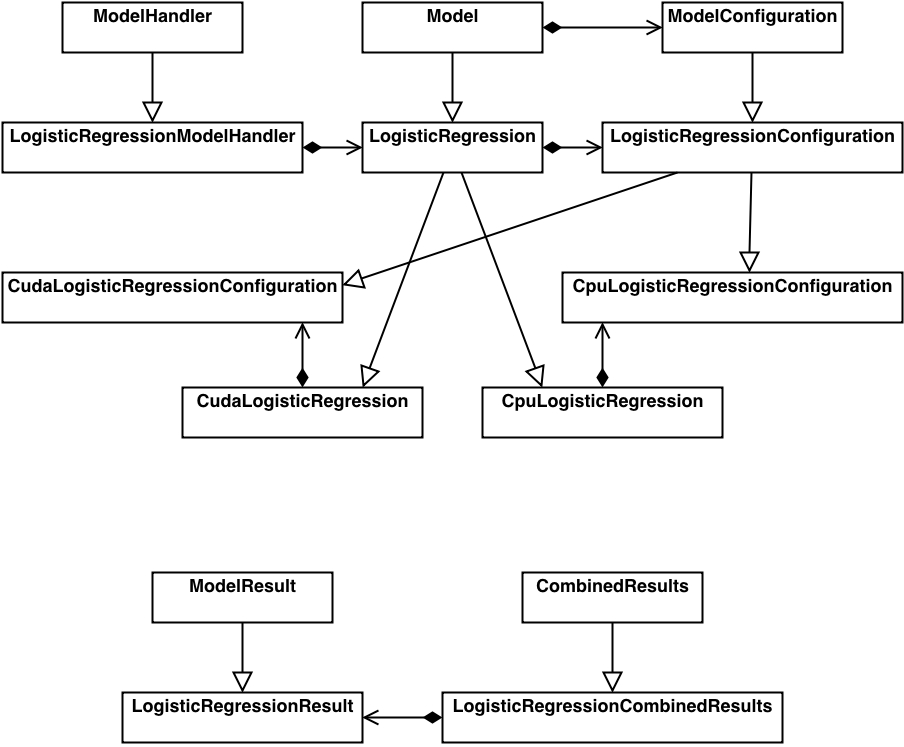
\includegraphics[width=12cm]{lr_structure.png}
    \caption{Overview of the logistic regression classes. White arrow is inheritance. Diamond is that the class with the diamond has instances of the other class.}
    \label{fig:lr_inheritance}
\end{figure}

\begin{figure}[h]
    \centering
    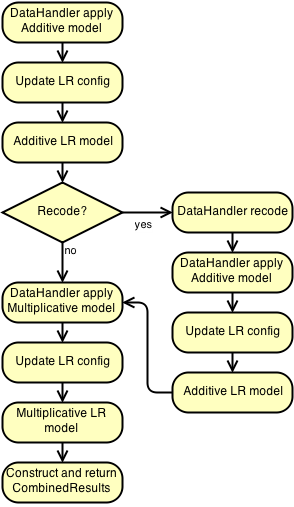
\includegraphics[width=6cm]{modelhandler_lr_layout.png}
    \caption{Layout of the LogisticRegressionModelHandler}
    \label{fig:lr_modelhandler}
\end{figure}

The LR algorithm is split into several protected functions so that each part can be tested individually. The parts are then used in the \textbf{calculate} function. For \textbf{CudaLogisticRegression} the parts corresponding to line 10 and 11 in algorithm \ref{alg:lr} are done on the host. All the other parts of the LR algorithm are done by using CUBLAS or the kernels explained in section \ref{kernelwrapper}. The calculations for line 10 and 11 are in the \textbf{LogisticRegression} class so the code is shared between \textbf{CpuLogisticRegression} and \textbf{CudaLogisticRegression}.\\
\\
Line 10 and 11 are done on the host instead of the device because the inverse of the information matrix(variable \textbf{J} in the algorithm) is done by SVD and no suitable GPU function for it was found. The reason for using SVD instead of normal matrix inverse was previously explained in section \ref{logistic_regression}. CUBLAS does not provide an SVD function. However there are other libraries that do, CULA Tools\cite{culatools} and MAGMA\cite{magma_2010}, however neither could be used.\\
\\
CULA Tools could not be used because it uses streams internally in the functions so it can not be executed on streams\cite{cula_forum_q}. It also uses device synchronisation which means that the all streams will be synchronised every time the function is used\cite{cula_forum_q}. MAGMA can use streams for its BLAS functions, however it does not for the other functions including the SVD\cite{magma_stream}.\\
\\
The size of the vectors and matrices used in that part are also small, their size is 4 + the number of covariates. However it can sometimes be better to calculate even small matrices and vectors on the device to avoid the transfers that would be needed otherwise\cite{cuda_best_practice}. An suitable GPU SVD kernel might be faster.\\
\\
After transfers it is necessary to wait for it to finish to prevent errors with using the data before it has been transferred completely. This is done by syncing the thread with the stream, it forces the thread to wait until all current kernels and transfers on the stream is complete. However due to the problem with asynchronous transfers and older architectures described in section \ref{streams} there is also an option when compiling to synchronise after each kernel.

\subsection{Worker Thread}
A number of worker threads use the previously explained classes to perform the work. One worker thread corresponds to one stream on a GPU. Normally three streams are used per GPU but it can easily be changed by changing a parameter in the main \textbf{Configuration} class. The layout of the worker thread is shown in figure \ref{fig:thread_layout}.\\
\\
The thread has its own \textbf{DataHandler}, \textbf{ModelHandler}, \textbf{ModelConfiguration} and Model. Some objects are shared with the other workers, most notably the \textbf{ResultFileWriter} and the \textbf{DataQueue}. Each thread loops over the \textbf{ModelHandlers} \textbf{next} function, tells the \textbf{ModelHandler} to calculate and then sends the results to the \textbf{ResultFileWriter}.

\begin{figure}[h]
    \centering
    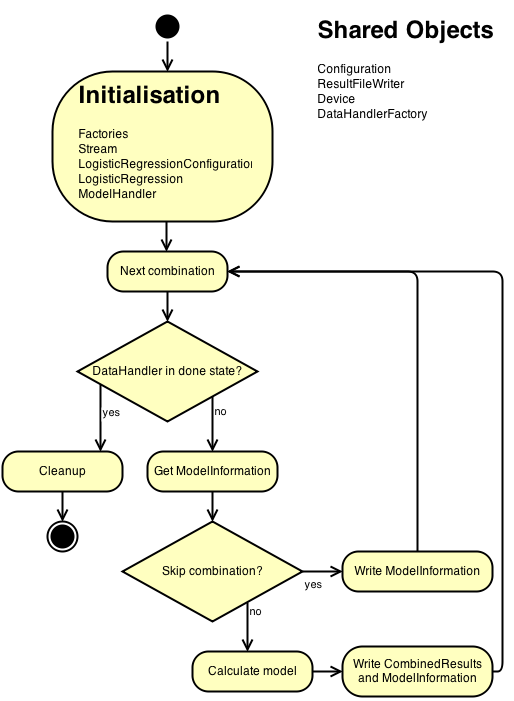
\includegraphics[width=10cm]{thread_layout.png}
    \caption{Structure of the worker thread}
    \label{fig:thread_layout}
\end{figure}

\subsection{Testing}
Almost all classes have a corresponding unit test that tests its functionality in isolation. However the matrix and vector classes are never mocked out because they are too basic and fundamental. It does mean that if there are multiple errors when testing and the tests for the matrix and vectors failed the fault likely is with those. However the number of integration tests are few and there is a need to create more.\\
\\
Since mocks are created by inheritance from the class to be mocked all functions need to be virtual. Some classes also have empty protected constructors to be used by the mock, others have helper functions to construct the mock. This goes against some parts of clean code but is necessary because of how C++ and mocking works. It could potentially be improved by using private constructors and friends to give the mock access.\\
\\
The data for the tests where calculated by hand or by using Matlab.

\subsection{Memory Usage}
The memory usage is low because only the SNPs whose models currently is being calculated is stored in memory. This also means that most of the memory usage depends on the number of individuals not the number of SNPs especially since the SNP class is small. The memory is also bound by the GPU rather than host memory because of the relative larger size of the host memory. The amount used depends on the precision, single precision floating point numbers are four bytes while double precision numbers are eight bytes.

\subsubsection{Device Memory}
%TODO fix intro
A Tesla GPU has 6 GB of memory\cite{nvtesla}.
The variables used on the device and their number of elements are shown in table \ref{table:gpu_variable_sizes}. The amount of individuals than can fit inside 6GB of memory for different number of covariates and precision is shown in table \ref{table:gpu_mem}.\\
\\

\begin{table}[h]
\begin{tabular}{| l c c |}
  \hline
  Matrix/vector & Size & Instances\\
  \hline
  Outcomes & $N$ & 1 \\
  Predictors & $N \times M$ & One per stream \\
  Probabilities & $N$ & One per stream \\
  Scores & $M$ & One per stream \\
  Beta & $M$ & One per stream \\
  Work Area & $N$ & One per stream \\
  Work Area & $N \times M$ & One per stream \\
  Information Matrix & $M \times M$ & One per stream \\
  \hline  
\end{tabular}
\caption{Sizes of the variables stored on the device, $N=$ number of individuals, $M=4+$ number of covariates}
\label{table:gpu_variable_sizes}
\end{table}

%Breaking out n
%\begin{equation}
%n=\frac{\frac{6GB}{6m+7}-m^2-6m}{precision}
%\end{equation}

\begin{table}[h]
\begin{tabular}{| l | l l |}
  \hline
  Number of covariates & Single precision & Double precision\\
  \hline
  0 & 48.4 & 24.2 \\
  5 & 24.6 & 12.3 \\
  10 & 16.5 & 8.2 \\
  20 & 9.0 & 5.0 \\
  100 & 2.4 & 1.2 \\
  \hline  
\end{tabular}
\caption{The number of individuals in millions needed to fill 6GB with the given precision, number of covariates and three streams.}
\label{table:gpu_mem}
\end{table}

\subsubsection{Host Memory}
%TODO host memory

N individuals
S snps
E env
C cov

\begin{table}[h]
\begin{tabular}{| l c c |}
  \hline
  Matrix/vector & Size & Instances\\
  \hline
  Outcomes & $N$ & 1 \\
  Environment data & $N \times E$ & 1 \\
  Covariates data & $N \times C$ & 1 \\
  SNPVector & $2N$ & One per stream \\
  EnvironmentVector & $N \times M$ & One per stream \\
  InteractionVector & $N \times M$ & One per stream \\
  Beta & $M$ & One per stream \\
  Scores & $M$ & One per stream \\
  Sigma & $M$ & One per stream \\
  uSVD & $M \times M$ & One per stream \\
  vSVD & $M \times M$ & One per stream \\
  Work area & $M \times M$ & One per stream \\
  \hline  
\end{tabular}
\caption{Sizes of the matrix/vector variables stored on the host}
\label{table:host_mv_variable_sizes}
\end{table}

\begin{table}[h]
\begin{tabular}{| l c c |}
  \hline
  Object & Size & Number\\
  \hline
  SNP & a & $S$\\
  EnvironmentFactor & a & $E$\\
  Persons & a & $N$\\
  \hline  
\end{tabular}
\caption{Sizes of the other stuff variables stored on the host}
\label{table:host_variable_sizes}
\end{table}


snp
string
vector int max l�ngd=4
string
string
int
int
bool
%=27+3*string

envfactor
string
int
%=4+string

person
string
int
int 
bool
%=9+string

The strings are short but there is significant overhead probably.

%p*n+s*(27+3*string)+e*(4+string)+n*(9+string)+p*n*e+p*n*c+3*4*p*(4*n+(4+c)*3+(4+c)^2*3)

alt form:
%c*(36*c*p+n*p+324*p)+n*(p*e+49*p+9)+string*(n+e+3*s)+720*p+4*e+27*s

\chapter{Results}
Intro\\
\\

\section{Data}
Acpapos

Simulated data, random, varying sizes
python script

\section{Hardware Specifications}
Cluster Zorn at PDC was used\cite{zorn_pdc}.

Zorn specs

8 nodes
92 gb ram
2 Intel Xeon E5620, 2.4 ghz, 4 cores
3 tesla m2090

Due to errors only one 1 GPU can be accessed. Because of this the login node had to be used for testing with multiple GPUs. It's specs are

%login node
4 tesla c2050
50 gb ram?

farliy old gpus

\newpage
\section{First look at speed}

\begin{figure}[h]
    \centering
    \includegraphics[width=9cm]{a1.png}
    \caption{Speedup vs 1 GPU on login node. 10 000 SNPs.}
    \label{fig:speed}
\end{figure}

\section{More detailed CuEira stuff}

for satured streams:
speedup for gpu

%\begin{figure}[h]
%    \centering
%    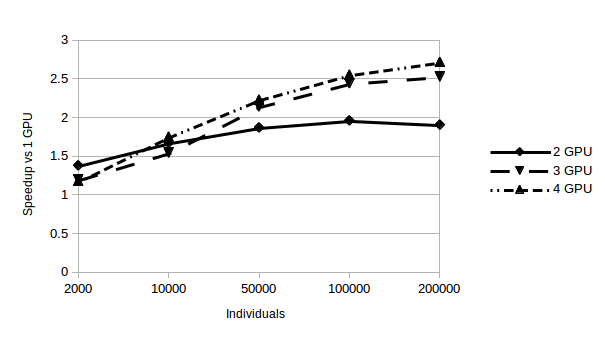
\includegraphics[width=12cm]{cueira_speedup_vs_1gpu_nocluster_10ksnps.png}
%    \caption{Speedup vs 1 GPU on login node. 10 000 SNPs.}
%    \label{fig:speedup_vs_1gpu}
%\end{figure}

efficency

%\begin{figure}[h]
%    \centering
%    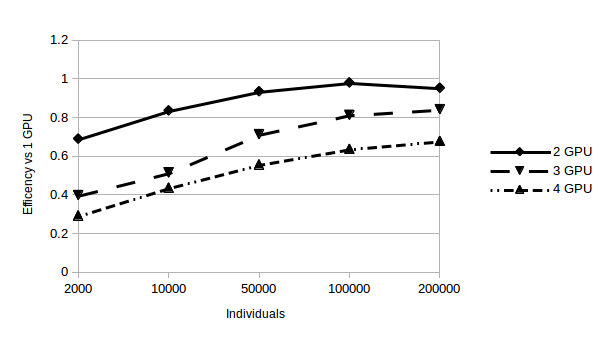
\includegraphics[width=12cm]{cueira_efficency_vs_1gpu_nocluster_10ksnps.png}
%    \caption{Efficiency vs 1 GPU on login node. 10 000 SNPs.}
%    \label{fig:efficency_vs_1gpu}
%\end{figure}

\section{Number of streams}
vary number of streams

\section{Single vs Double Precision}
time increased slightly for double

%\begin{figure}[h]
%    \centering
%    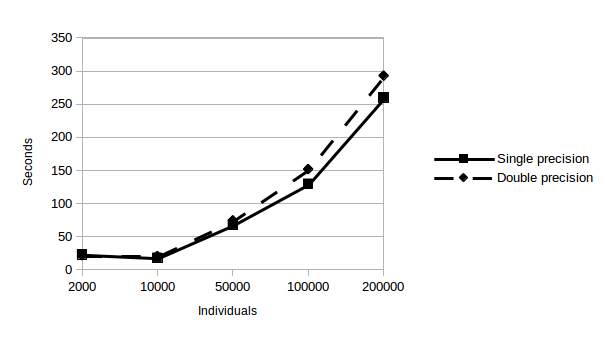
\includegraphics[width=12cm]{single_vs_double_10ksnps_4gpu.png}
%    \caption{Execution time with 4 GPUs with either single or double precision. 10 000 SNPs.}
%    \label{fig:single_vs_double_10ks_4gpu}
%\end{figure}

%\begin{figure}[h]
%    \centering
%    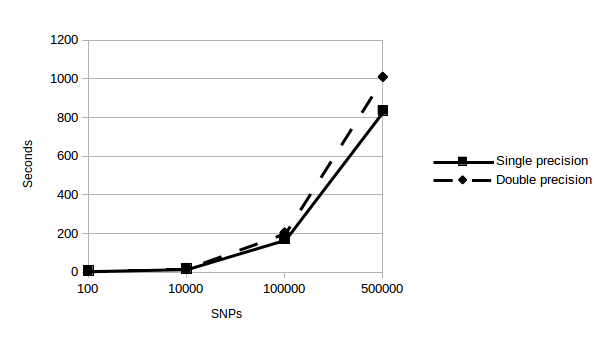
\includegraphics[width=12cm]{single_vs_double_10ki_4gpu.png}
%    \caption{Execution time with 4 GPUs with either single or double precision. 10 000 individuals.}
%    \label{fig:single_vs_double_10ki_4gpu}
%\end{figure}

%\begin{figure}[h]
%    \centering
%    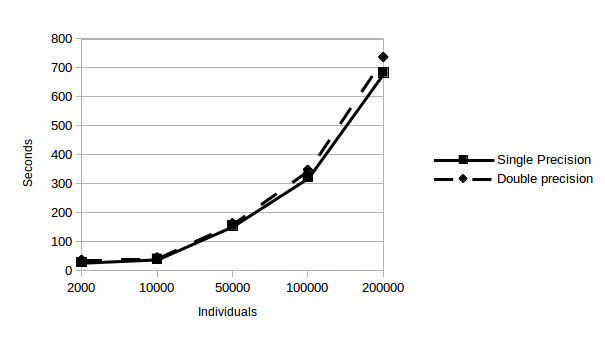
\includegraphics[width=12cm]{single_vs_double_10ks_cluster.png}
%    \caption{Execution time with 1 GPU on login node with either single or double precision. 10 000 SNPs.}
%    \label{fig:single_vs_double_10ks_cluster}
%\end{figure}

%\begin{figure}[h]
%    \centering
%    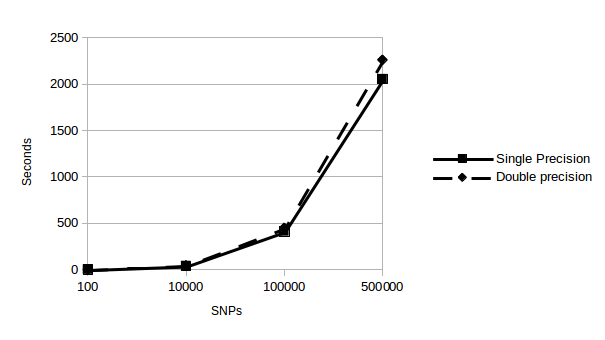
\includegraphics[width=12cm]{single_vs_double_10ki_cluster.png}
%    \caption{Execution time with 1 GPU on login node with either single or double precision. 10 000 individuals.}
%    \label{fig:single_vs_double_10ki_cluster}
%\end{figure}

\section{Syncing}
%kepler vs fermi queue problem, problem described in section \ref{streams}
minor increase with syncing

%\begin{figure}[h]
%    \centering
%    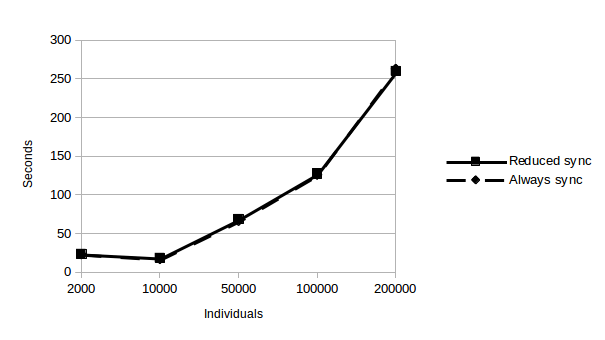
\includegraphics[width=12cm]{ferm_vs_nofermi_10ksnps_4gpu.png}
%    \caption{Execution time with 4 GPUs with either synchronisation or not. 10 000 SNPs.}
%    \label{fig:sync_vs_no_sync_4gpu_10ks}
%\end{figure}

%\begin{figure}[h]
%    \centering
%    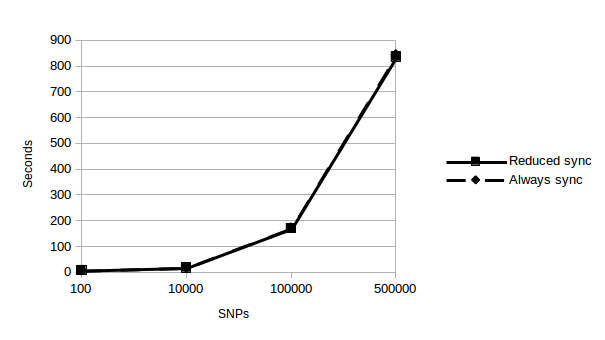
\includegraphics[width=12cm]{ferm_vs_nofermi_10ki_4gpu.png}
%    \caption{Execution time with 4 GPUs with either synchronisation or not. 10 000 individuals.}
%    \label{fig:sync_vs_no_sync_4gpu_10ki}
%\end{figure}

%\begin{figure}[h]
%    \centering
%    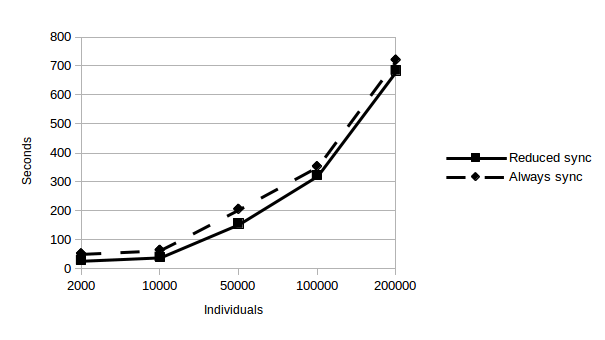
\includegraphics[width=12cm]{ferm_vs_nofermi_10ks_cluster.png}
%    \caption{Execution time with 1 GPU on cluster node with either synchronisation or not. 10 000 SNPs.}
%    \label{fig:sync_vs_no_sync_cluster_10ks}
%\end{figure}

%\begin{figure}[h]
%    \centering
%    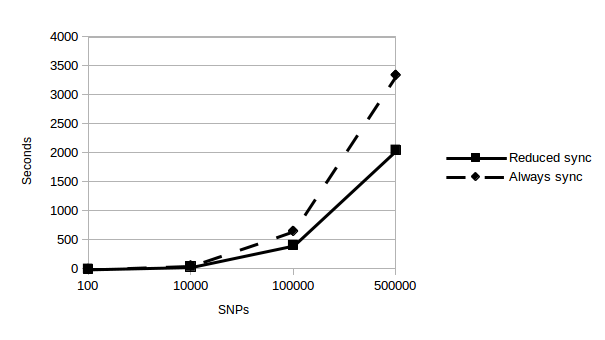
\includegraphics[width=12cm]{ferm_vs_nofermi_10ki_cluster.png}
%    \caption{Execution time with 1 GPU on cluster node with either synchronisation or not. 10 000 individuals.}
%    \label{fig:sync_vs_no_sync_cluster_10ki}
%\end{figure}

\section{Profiling}
The reading of the fam file sometimes takes several seconds. It seems to happen with smaller files, no big deal

Because of asynchronous and threads can be hard to draw conclussions even if one part takes time. Because can be hidden by GPU

time spent at various parts
1/2 gpu vs 4 gpu, cpu vs gpu on LR

nsight, 100 snps, 2 gpu vs 4 gpu sync/vs no sync

\subsection{Locks}
The \textbf{ResultFileWriter} and \textbf{DataQueue} each has a lock to prevent race conditions. They also have a timer for how much time that has been spent waiting at the locks. 

There was very little time spent at the locks, not more than a couple of seconds even for the larger files.
good because clusters later

\subsection{ModelHandler and DataHandler}
some time on recode and app model

however signficant on reading snp

plot time \% spent

\subsection{LR}
additional syncs because of the timers to be accurate

does it affect?

\section{Compiler Optimizations}
no aliasing
for both cuda and host

fast math cuda

-opt2 vs opt3

mkl parallel vs sequential

\chapter{Discussion and Conclusions}
%Discussion and Conclusions (up to 3 pages)
%Need for novel methods for gene-environment interaction
%Need for methods for third order interaction and higher
%more statistics for non binary

\section{Scaling}

snp scaling
double the snps doulbe the calc time
because completely independent

individual scaling

covariates scaling
non linear, since lot of matrix stuff

\section{Saturation of CPU}
saturation of the cpus seems to have large impact
shows with 4 gpu=12 streams>8 cores
or with 1 gpu 1 stream vs 1 gpu 4 stream

solution:more stuff to gpu, the SVD and the recoding
->much less transfers

if there is cpu power left could use separate cpu worker threads to fill the rest, cpu version is good to have too

add mpi support and use several nodes

split out the snp reading to separate threads. add another queue. 

%TODO look back att efficent cuda part

%TODO divergence problems, nothing now but could be with recoding on GPU or bootstrap
%idea for solution using pointer architmic

%need to change mkl to any blas and remove dependency on intel compiler

%amdahl vs gustafson, gustafson probably more right on this stuff since with more power data can increase. also even without larger data there is higher order interactions

%recoding on GPU instead of cpu

%clusters
%kinda possible by splitting the input files

%cublas not that much harder than regular blas. A wrapper could enable simple and easy use without losing too much features.
%however will get problems with large data amounts, can't fit in device memory
%own kernels more than simple elemntwise, probably hard to optimize. unknowish

\section{Extending Additive Interaction to Non Binary}
More statistics needed 

OR>1 because recoding, see section \ref{recode}

\begin{equation}
OR_{both\:factors\:present}^x>OR_{first\:factor\:present}+OR_{second\:factor\:present}^x-1
\end{equation}
Where x is the number of steps from the base level.

This means that the interaction depends on the level of the factor. There are four cases

Using $\beta_{snp}$
$\beta_{environment}$
$\beta_{interaction}$

\begin{table}[h]
\begin{tabular}{| l | l | l |}
  \hline
  Case & Additive Interaction present, binary factor & Additive interaction present, non binary factor\\
  \hline
  $\beta_{interaction}>\beta_{snp} \; \beta_{interaction}>\beta_{environment}$ & Yes & Yes\\
  $\beta_{interaction}<\beta_{snp} \; \beta_{interaction}<\beta_{environment}$ & No & No\\
  $\beta_{interaction}>\beta_{snp} \; \beta_{interaction}<\beta_{environment}$ & No & For some x\\
  $\beta_{interaction}<\beta_{snp} \; \beta_{interaction}>\beta_{environment}$ & No & For some x\\
  \hline  
\end{tabular}
\caption{Additive interaction cases for non binary environmental factor}
\label{table:additive_interaction}
\end{table}

Can also be written as

\begin{equation}
OR_{both\:factors\:present}^x-OR_{second\:factor\:present}^x>OR_{first\:factor\:present}-1
\end{equation}

In case 3 it is monotone increasing

In case 4 it is monotone decreasing

%TODO make some plots of it

Which means both pass 0 at one point.(Unless all equal 1 which means all 0)

That point can be found by solving

\begin{equation}
OR_{both\:factors\:present}^x-OR_{second\:factor\:present}^x=+OR_{first\:factor\:present}-1
\end{equation}

Case 3 has interaction for x>the point
Case 4 has interaction for x<the point

However case 4: point x=0 is at 0? x=1 is <0 so no point >0 after x>0
So only case 3

Depending on where the point is interaction might not be relevant, e.g. needs to smoke a million cigarettes a day and case 3. Or disappears to fast, eg 1 cigarette a year case 4.

Since the odds is an monotone function, switching lowest risk with highest means inverting the interval of the variable, e.g. minimum becomes maximum, maximum becomes minimum.


\chapter{Outlook}
%Outlook (up to one page)

%more statistics for non binary
%if binary possibly take inspiration from g-g?

gpus good for interaction, how about xeon phi?
depends on method, some methods diverge and stuff, for instance article thingy uses GPU but has divergence stuff, maybe xeon phi/cpu cluster better for them?

small parts on cpu, not so good

\newpage
\bibliographystyle{ieeetr}
\bibliography{hpc.bib,statistics.bib,misc.bib}

\begin{appendices}

\chapter{Lists}

\addcontentsline{toc}{section}{List of Abbreviations}
\section*{List of Abbreviations}

\begin{description}
\item[MAF] \hfill \\
  Minor allele frequency, the frequency of the least common allele.
\item[RF] \hfill \\
  Random Forest
\item[MDR] \hfill \\
  Random Forest
\item[OR] \hfill \\
  Random Forest
\item[RR] \hfill \\
  Random Forest
\item[RERI] \hfill \\
  Random Forest
\item[AP] \hfill \\
  Random Forest
\item[SI] \hfill \\
  Random Forest
\item[GPU] \hfill \\
  Random Forest
\item[CPU] \hfill \\
  Random Forest
\item[SM] \hfill \\
  Streaming multiprocessor
\item[SIMD] \hfill \\
  Random Forest
\item[MIMD] \hfill \\
  Random Forest
\item[SIMT] \hfill \\
  Random Forest
\item[SISD] \hfill \\
  Random Forest
\item[LR] \hfill \\
  Random Forest
\item[MIDSD] \hfill \\
  Random Forest

% a t g c IDE SVD
\end{description}

\cleardoublepage
\addcontentsline{toc}{section}{List of Algorithms}
\listofalgorithmslist

\cleardoublepage
\addcontentsline{toc}{section}{List of Examples}
\listofexample

\cleardoublepage
\addcontentsline{toc}{section}{List of Figures}
\listoffigures

\cleardoublepage
\addcontentsline{toc}{section}{List of Tables}
\listoftables

\chapter{File Formats}
\label{file_formats}

\section{PLINK Data Format}
\label{plink_file}
%TODO plink file stuff

The PLINK files can be in different formats. 

The binary format consists of three files. Bed, bim and fam. The 

\cite{plink_format}

\section{Environmental and Covariates File Format}
The environmental factors and covariates are stored in separate files with the same format, one file for environmental factors and one for the covariates if any. One of the columns needs to contain the individual ids, the rest of the columns should be data. The delimiter can be any reasonable string(e.g. something that is not part of a name or number) and there is an option to set the delimiter in the program. The default is tab delimited.

\section{CuEira Result File Format}
The results from CuEira are written in an csv file. It has 48 columns described below.

\begin{description}
\item[snp\_id] \hfill \\
  The id of the SNP from the bim file.
\item[pos] \hfill \\
  The row which the SNP had in the plink files.
\item[skip] \hfill \\
  Numbers explaining why the SNP was excluded from calculation. 1=missing data. 2=low MAF, 3=low cell count, 4=negative position in bim file
\item[risk\_allele] \hfill \\
  The risk allele, not changed based on recoding
\item[minor] \hfill \\
  The minor allele
\item[major] \hfill \\
  The major allele
\item[env\_id] \hfill \\
  The id of the environment factor, it is the column form the environment file.
\item[no\_alleles\_X] \hfill \\
  The numbers of the alleles in group X
\item[freq\_alleles\_X] \hfill \\
  The frequencies of the alleles group X
\item[no\_snpX\_envY] \hfill \\
  Cell distribution with exposure X and Y.
\item[ap] \hfill \\
  The AP value for the additive model described in \ref{statistic_measures}
\item[reri] \hfill \\
  The RERI value for the additive model described in \ref{statistic_measures}
\item[OR] \hfill \\
  The odds ratios for the SNP, environment factor and interaction. Add is for the additive model and mult is for the multiplicative. L is the lower confidence interval and H is the upper. The interval is from using the delta method\cite{uvehag_master_thesis}.
\item[recode] \hfill \\
  Case of recoding, 0=no recoding, 1=snp protective, 2=environment protective, 3=interaction protective
\end{description}

Each line after the header is a combination of a SNP and an environment factor. Because of the parallel nature of the program the rows are not in any specific order. The column pos contains the row number that the SNP had in the plink files. This can be used to sort the data in.\\
\\
The data in some columns are changed depending on the recoding. The multiplicative model is calculated using the recode from the additive model. The cell frequencies are also changed. However the risk allele is not changed.

\chapter{Risk Allele}
\label{risk_allele_appendix}
This appendix contains a more detailed look at different risk allele definitions than section \ref{risk_allele}.\
\\
The code for how JEIRA and GEISA calculates the risk allele is not the same as its definition \cite{geira, uvehag_master_thesis} talked about previously in section \ref{risk_allele}. The algorithm JEIRA and GEISA uses is shown in algorithm \ref{alg:jeira_geisa_risk_allele}.

\begin{algorithm}
\DontPrintSemicolon
\SetKwInOut{data}{Data}
\BlankLine \BlankLine

\data{
$caseMaxAllele$ is the most common allele in case and $controlMaxAllele$ is the most common in control\\
$caseMaxRatio$ and $controlMaxRatio$ is the frequency of $caseMaxAllele$ and $controlMaxAllele$ respectively.\\
}

\BlankLine \BlankLine

\If{$caseMaxRatio > controlMaxRatio$ \KwSty{and} $caseMaxAllele=controlMaxAllele$}{
  $riskAllele \longleftarrow caseMaxAllele$\;
}\Else{
  $riskAllele \longleftarrow caseMinAllele$\;
}

\caption{JEIRA and GEISA pseudo code to determine the risk allele}
\algorithmslist{\quad JEIRA and GEISA pseudo code to determine the risk allele}
\label{alg:jeira_geisa_risk_allele}
\end{algorithm}

The allele frequencies can be shown in an $2 \times 2$ table. The columns are the frequencies for the different alleles and the rows are the groups(case and control). It can be split into four cases shown in table \ref{table:risk_allele_cases}. The four cases comes from the four cases of possible directions of the inequality between the maximum frequencies of the two groups. There is up, down, down diagonally and up diagonally. The rest of the inequalities can be found by using that the sum of each row is 1.\\

\begin{table}[h]
\centering
\begin{tabular}{| l | c c c | c | c c c |}
  \hline
   & Allele1 & & Allele2 & & Allele1 & & Allele2  \\
  \hline
  Case & Max & $\rightarrow$ & Min & & Max & $\rightarrow$ & Min \\
   & \textcolor{arrow}{$\downarrow$} & $\nese$ & $\uparrow$ & & \textcolor{arrow}{$\uparrow$} & $\nese$ & $\downarrow$ \\
  Control & Max & $\rightarrow$ & Min & & Max & $\rightarrow$ & Min \\
  \hline 
  & & & & & & &\\
  \hline
  Case & Max & $\rightarrow$ & Min & & Max & $\rightarrow$ & Min \\
   & $\downarrow$ & $\nesecol$ & $\uparrow$ & & $\downarrow$ & $\nwsw$ & $\uparrow$ \\
  Control & Min & $\leftarrow$ & Max & & Min & $\leftarrow$ & Max \\
  \hline  
\end{tabular}
\caption{The four cases of allele frequencies}
\label{table:risk_allele_cases}
\end{table}
%TODO clarify which case is which

By using the previously mentioned definitions in section \ref{risk_allele} and the JEIRAs and GEISAs algorithm \ref{alg:jeira_geisa_risk_allele} what the risk allele is according to them for each case is shown in table \ref{table:risk_allele_comp}. Each definition correspond to examining the inequalities in the cases. For the definition using MAF the direction of the inequality from case minimum to control minimum determines it. If it points towards control the the case minor allele is the risk allele. For JEIRA and GEISA if the maximum for case points straight down to the maximum for control then the major case allele is the risk allele. This only happens in case 1. For increased frequency in case it is the allele which has the inequality pointing straight down.\\

\begin{table}[h]
\centering
\begin{tabular}{| l | c c c c |}
  \hline
  Definition & Case 1 & Case 2 & Case 3 & Case 4  \\
  \hline
  MAF based & Allele1 & Allele2 & Allele1 & Allele2 \\
  JEIRA GEISA algorithm & Allele1 & Allele2 & Allele2 & Allele2 \\
  Increase frequency in case & Allele1 & Allele2 & Allele1 & Allele1 \\
  \hline  
\end{tabular}
\caption{Risk alleles for the cases in table \ref{table:risk_allele_cases} based on the different definitions}
\label{table:risk_allele_comp}
\end{table}

The risk allele is different for case 3 and case 4. For case 3 it is clear that it should be Allele1 because it has the highest frequency in case and also higher in case than control An extreme case of case 3 is shown in table \ref{table:risk_allele_extreme_case_3}.\\
\\
By examining a similar extreme case of case 4 it is clear that Allele1 should be the risk allele in that case too. The case is shown in table \ref{table:risk_allele_extreme_case_4}. Almost everyone in the case group has Allele1 while no one in the control group does, it is unlikely that Allele2 would increase the risk in that case.

\begin{table}[h]
\centering
\begin{tabular}{| l | c c |}
  \hline
   & Allele1 & Allele2  \\
  \hline
  Case & 1 & 0.00  \\
  Control & 0.01 & 0.99\\
  \hline  
\end{tabular}
\caption{An extreme case of frequencies of case 3 in table \ref{table:risk_allele_cases}}
\label{table:risk_allele_extreme_case_3}
\end{table}

\begin{table}[h]
\centering
\begin{tabular}{| l | c c |}
  \hline
   & Allele1 & Allele2  \\
  \hline
  Case & 0.99 & 0.01  \\
  Control & 0 & 1  \\
  \hline  
\end{tabular}
\caption{An extreme case of frequencies of case 4 in table \ref{table:risk_allele_cases}}
\label{table:risk_allele_extreme_case_4}
\end{table}

\chapter{Bugs and Issues}
This is a small collection of various bugs and limitations encountered in the course of the project that can be good to know for anyone that wants to compile CuEira or if the libraries are used in other projects.

\section{Bugs}
\label{found_bugs}
There are several problems with Intel compilers and libraries. Most libraries work fine with gnu C/C++ compiler but have problems with Intel compilers. Boost 1.55 does not work with Intel compilers, 1.54 works. AllOf in Google Test also does not work together with Intel compilers.\\
\\
JEIRA prints the wrong results for the multiplicative model and as mentioned in appendix \ref{risk_allele_appendix} the risk allele algorithm JEIRA uses is not the same as the definition.

\section{Issues}
Nvcc can not compile c+11 code and no interface included in the code that nvcc compiles can use c++11. This problem can largely be avoided by using separate compilation. The CUDA find package module for CMake(included in version 2.8 and later) has a default flag that should be removed as it can cause problems. The flag tells nvcc to propagate the host code flags, if the compiler for the host code then uses c++11 that flag is propagated to nvcc and it will not compile The flag is disabled in CMake by using set(CUDA\_PROPAGATE\_HOST\_FLAGS off).

\chapter{How to Compile and Use CuEira}
\label{compile_cueira}
The source code for the program is available at github, \url{https://github.com/Berjiz/CuEira}.

\begin{description}
    \item[List of dependencies. Listed version is the version used.]
\end{description}
\begin{itemize}
 \item Boost, tested with version 1.54, 1.55 does not work due to a bug with Intel compilers
 \item CMake, version 2.8
 \item CUDA, version 5.5
 \item MKL, version 13.1
 \item Intel compiler version 14.0
 \item Google Test and Google Mock, already included in the folder.
\end{itemize}

First install the dependencies, they might need to be compiled from source. Open a terminal and make a new directory where you want the program to be compiled. Enter the directory and write:\\
cmake /path/to/CuEira/\\
Then type:\\
make\\
\\
The program should now be compiling. CMake might complain about not finding a dependency. If it does you need to tell CMake where it is. The path to boost is set by using EXPORT BOOST\_ROOT = /path/to/boost/. The path to the compilers is done with CXX = cmake /path/to/source for the C++ compiler and C = cmake /path/to/source for the C compiler.\\
\\

%TODO how to set cuda

In the build/bin directory there is two executable files, CuEira and CuEira\_Test. CuEira is the program itself while CuEira\_Test runs all the tests for the program. 
%TODO usage

\end{appendices}

\end{document}